\chapter{Desenvolvimento}\label{cap:desenvolvimento}

Este capítulo apresenta os artefatos produzidos durante a primeira \textit{sprint} do projeto, contemplando a modelagem inicial do sistema. Os elementos aqui descritos foram fundamentais para alinhar a visão da equipe em relação às funcionalidades, à interface do usuário e à estrutura do banco de dados.

\section{Diagrama de Casos de Uso}
O diagrama de casos de uso tem como objetivo ilustrar, de forma abstrata, as principais funcionalidades do sistema e os atores envolvidos. Este artefato permitiu identificar, já na fase inicial, quais interações devem ser suportadas pela aplicação.

\begin{figure}[H]
    \centering
    \includesvg[width=1\textwidth]{imgs/diagrama-casos-de-uso.svg}
    \caption{Diagrama de Casos de Uso do Sistema}
    \label{fig:casos_uso}
\end{figure}

\subsection{Descrição dos Casos de Uso}
\begin{itemize}
    \item \textbf{Entrar}:Permite que o usuário acesse o sistema utilizando suas credenciais (e-mail e senha).
    \item \textbf{Cadastrar}: Possibilita que novos usuários criem uma conta no sistema, informando seus dados básicos.
    \item \textbf{Visualizar Resumo Financeiro}: Exibe uma visão geral da situação financeira do usuário, incluindo saldo disponível, movimentações recentes, contas a pagar, patrimônio. Também mostra um gráfico que relaciona os bens e as despesas, e ainda permite ao usuário registrar despesas e entradas eventuais de maneira rápida.
    \item \textbf{Gerenciar Saídas}: Permite registrar, editar e excluir despesas. Inclui a categorização de gastos para facilitar a análise.
    \item \textbf{Gerenciar Contas Recorrentes}: Facilita o controle de despesas fixas, como contas de serviços públicos, aluguel, entre outras. Permite adicionar, editar e remover contas recorrentes.
    \item \textbf{Gerenciar Entradas}: Permite registrar, editar e excluir receitas. Inclui a categorização de entradas para facilitar a análise.
    \item \textbf{Gerenciar Patrimônio}: Possibilita o cadastro de bens, como imóveis, veículos ou outros ativos de valor, permitindo acompanhar sua valorização ou depreciação.
    \item \textbf{Gerenciar Investimentos}: Permite cadastrar, acompanhar e atualizar informações sobre investimentos. Inclui também a possibilidade de liquidar investimentos, registrando sua venda ou encerramento.
    \item \textbf{Gerenciar Conta}: Permite ao usuário atualizar suas informações pessoais, alterar a senha e excluir sua conta do sistema.
    \item \textbf{Sair}: Permite que o usuário encerre sua sessão no sistema de forma segura.
\end{itemize}

\section{Protótipos de Baixa Fidelidade}
Os protótipos de baixa fidelidade foram desenvolvidos para representar a organização e o fluxo das telas do sistema, servindo como base para discussões e refinamentos futuros. Essa etapa auxilia na antecipação de problemas de usabilidade e na validação das ideias de interface junto à equipe.

\begin{figure}[H]
    \centering
    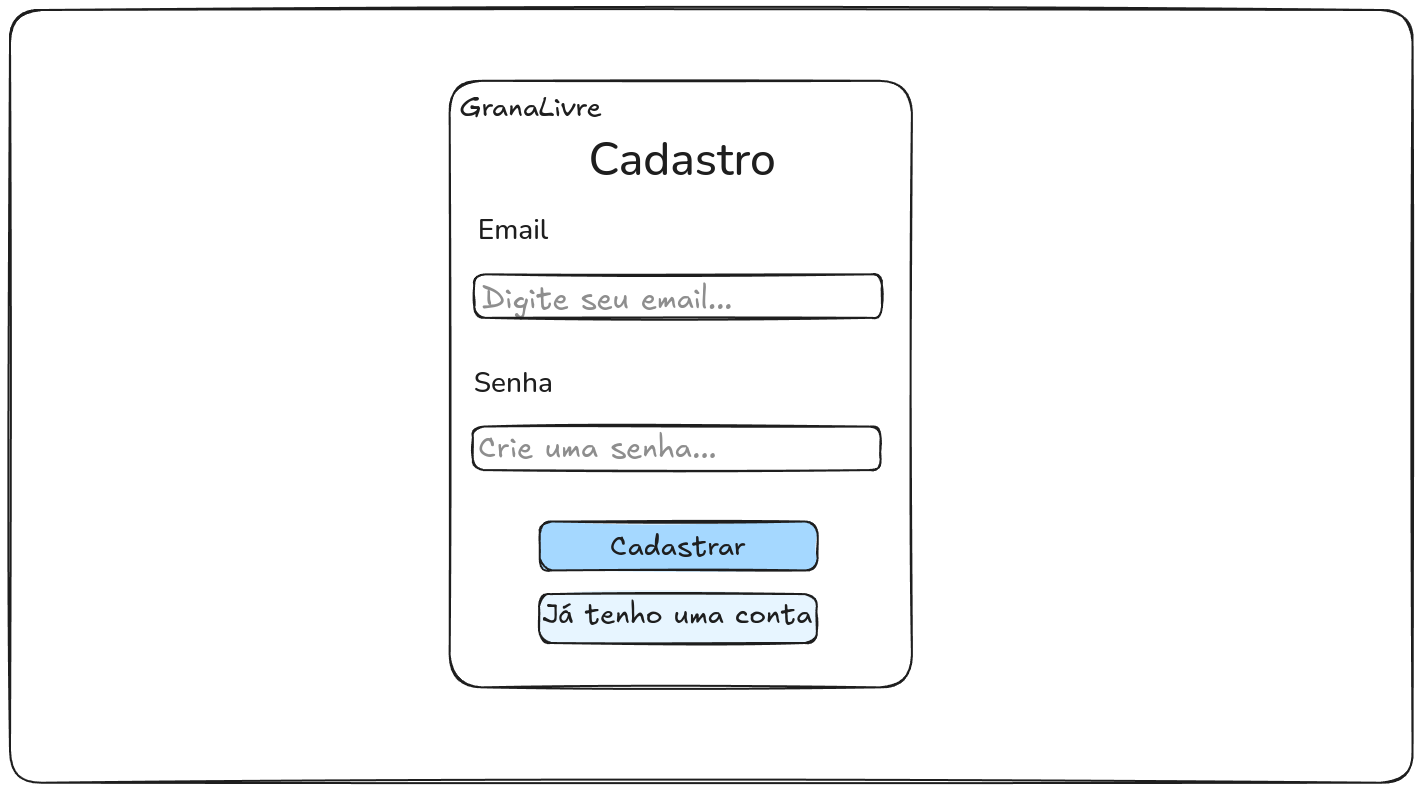
\includegraphics[width=0.9\textwidth]{imgs/01-cadastro.png}
    \caption{Protótipo de baixa fidelidade da tela de login}
    \label{fig:prot_login}
\end{figure}

\begin{figure}[H]
    \centering
    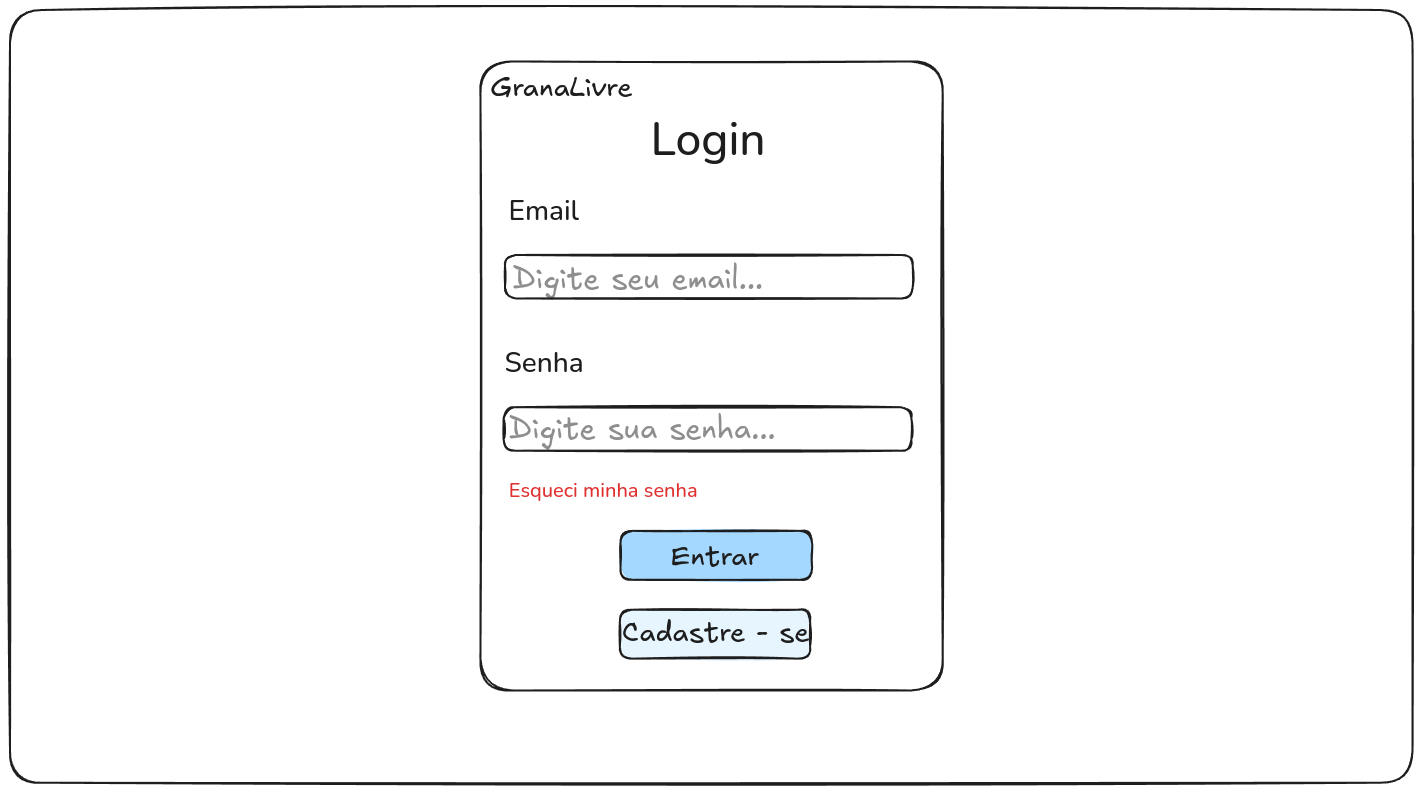
\includegraphics[width=0.9\textwidth]{imgs/02-login.png}
    \caption{Protótipo de baixa fidelidade da tela inicial}
    \label{fig:prot_inicial}
\end{figure}

% 03-resumo.png
\begin{figure}[H]
    \centering
    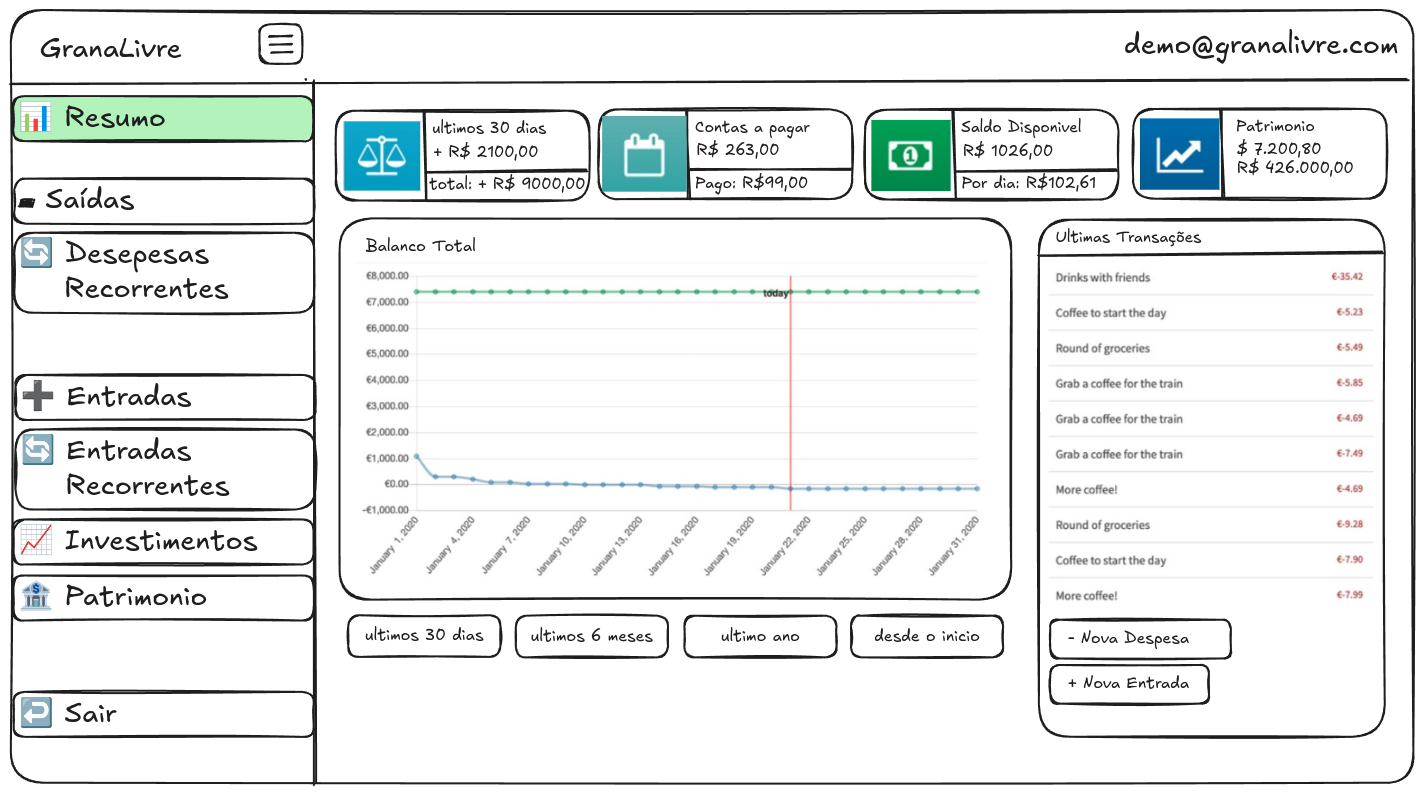
\includegraphics[width=0.9\textwidth]{imgs/03-resumo.png}
    \caption{Protótipo de baixa fidelidade da tela de resumo financeiro}
    \label{fig:prot_resumo}
\end{figure}

% 03-resumo2.png mostra botão com informações da conta do usuario
\begin{figure}[H]
    \centering
    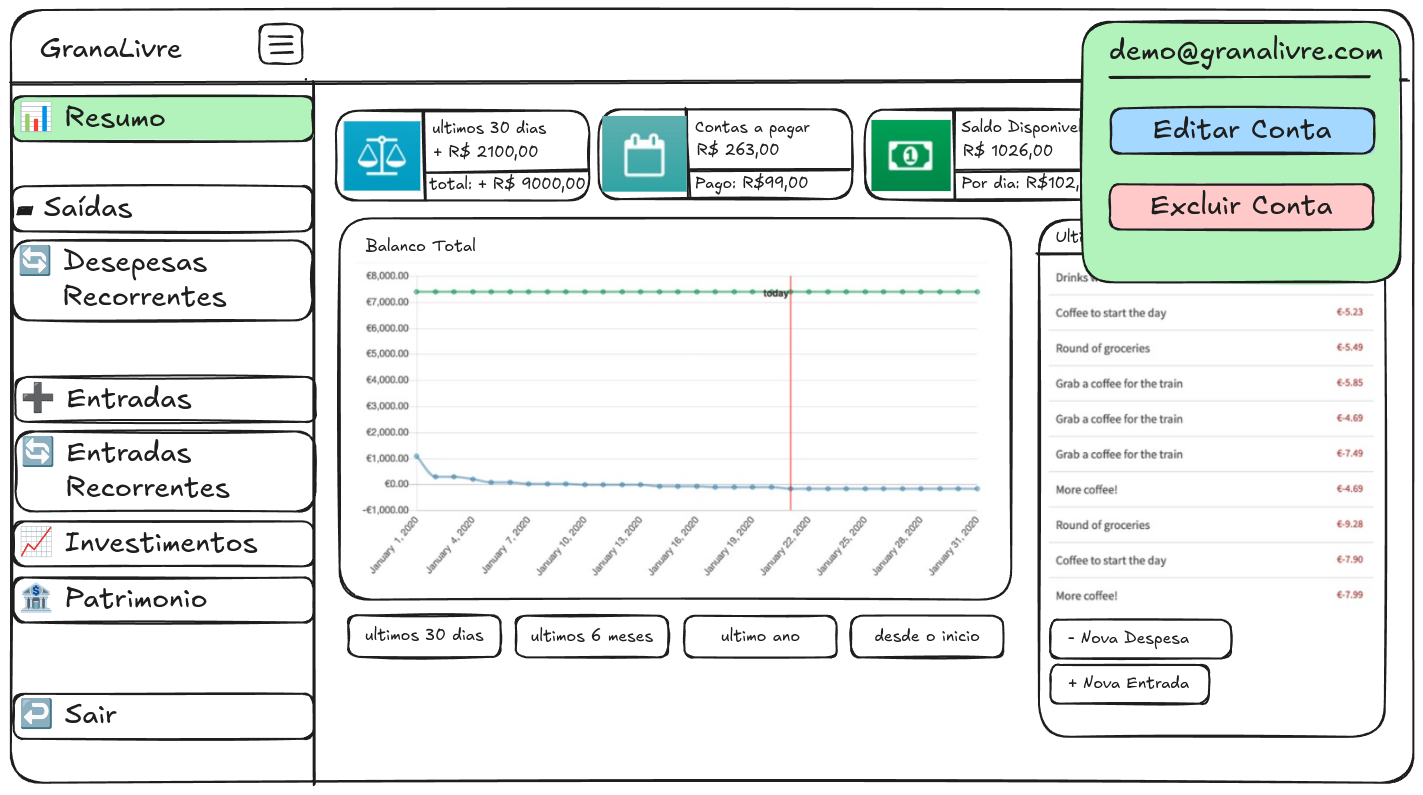
\includegraphics[width=0.9\textwidth]{imgs/03-resumo2.png}
    \caption{Protótipo de baixa fidelidade da tela de resumo financeiro com detalhes da conta do usuário}
    \label{fig:prot_resumo2}
\end{figure}

%03-resumo3.png editar informacoes da conta do usuario
\begin{figure}[H]
    \centering
    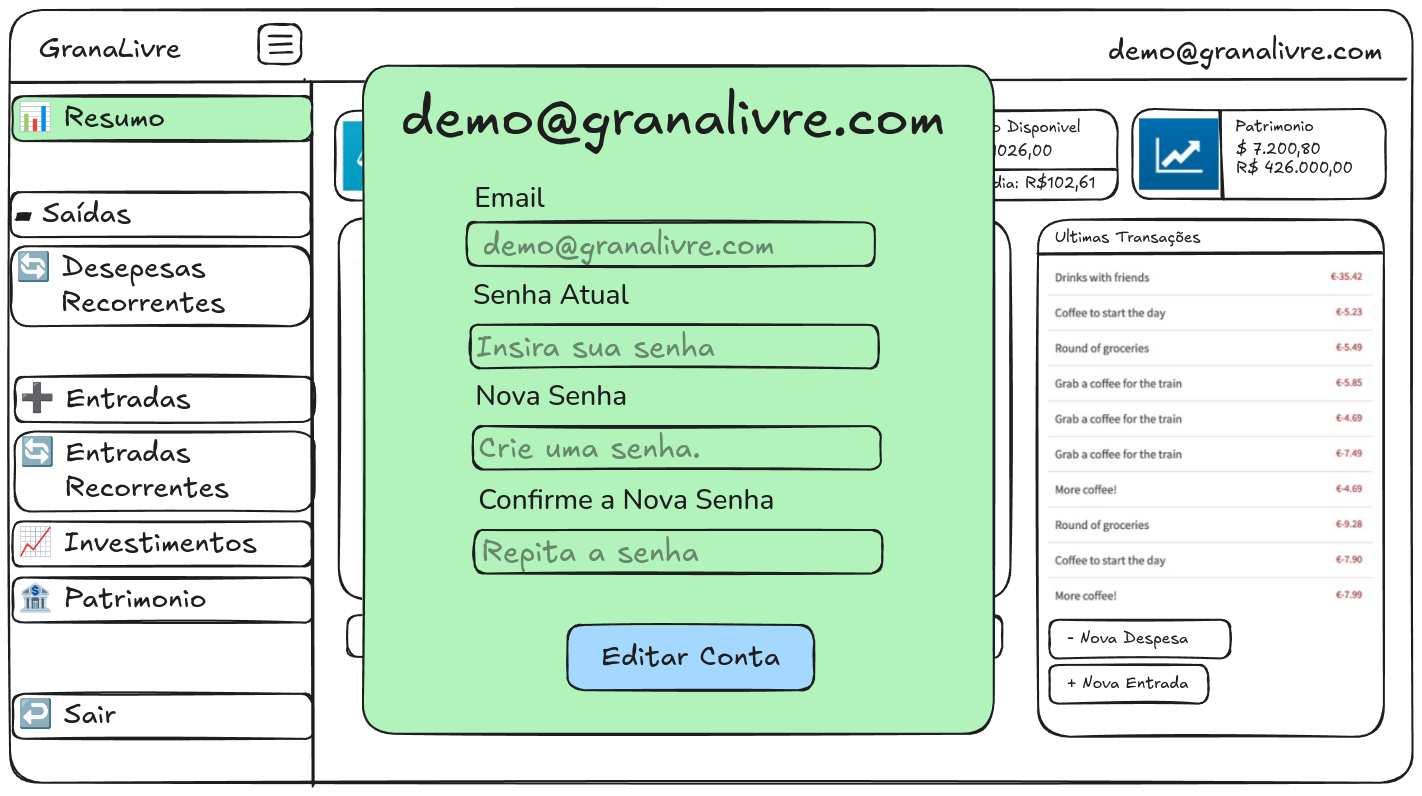
\includegraphics[width=0.9\textwidth]{imgs/03-resumo3.png}
    \caption{Protótipo de baixa fidelidade da tela de resumo financeiro com opção de editar informações da conta do usuário}
    \label{fig:prot_resumo3}
\end{figure}

%03-resumo4.png exclusao da conta do usuario
\begin{figure}[H]
    \centering
    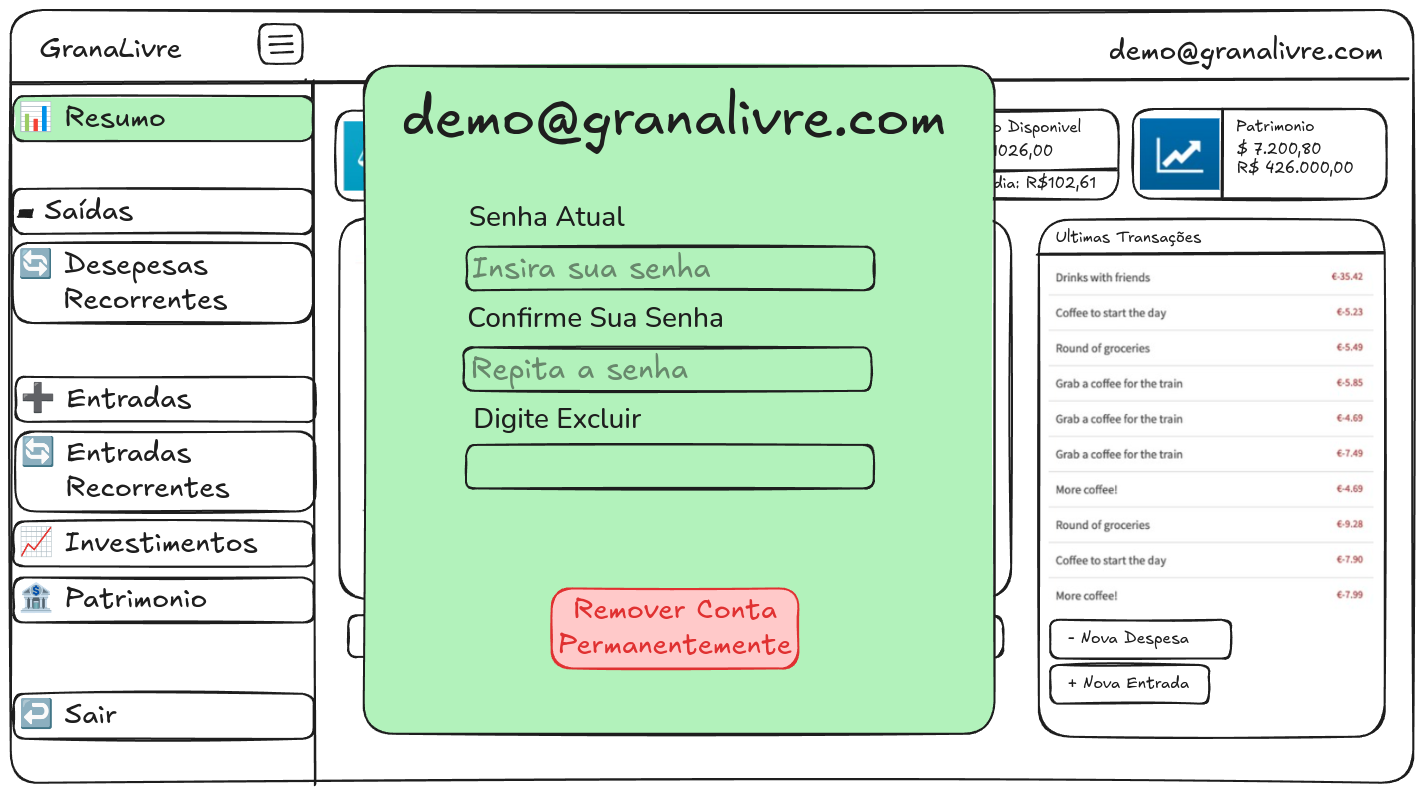
\includegraphics[width=0.9\textwidth]{imgs/03-resumo4.png}
    \caption{Protótipo de baixa fidelidade da tela de resumo financeiro com opção de exclusão da conta do usuário}
    \label{fig:prot_resumo4}
\end{figure}

%04-despesas_recorrentes até 04-despesas_recorrentes_4.png
\begin{figure}[H]
    \centering
    % \includesvg[width=1\textwidth]{imgs/04-despesas_recorrentes.svg}
    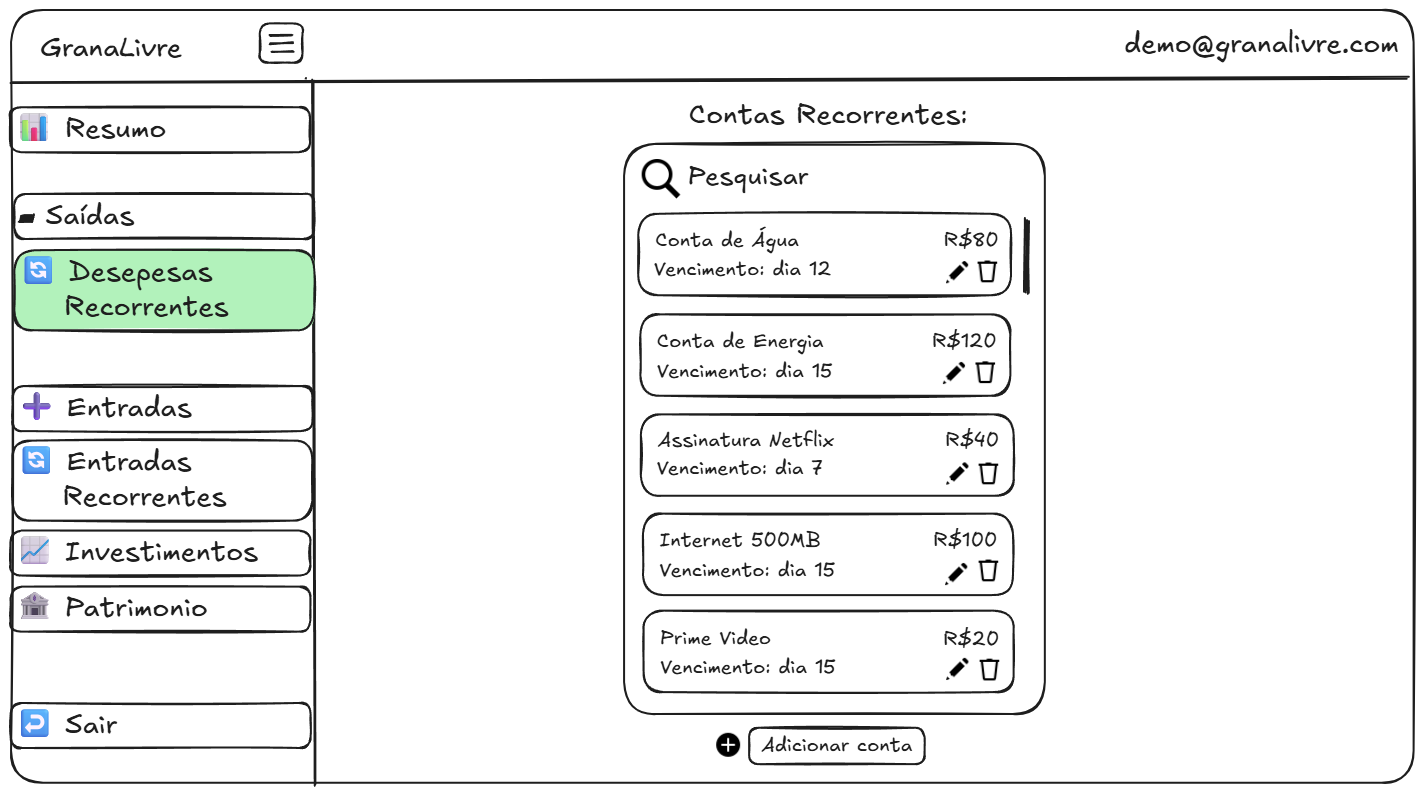
\includegraphics[width=0.9\textwidth]{imgs/04-despesas_recorrentes.png}
    \caption{Protótipo de baixa fidelidade da tela de gerenciamento de despesas recorrentes}
    \label{fig:prot_despesas_recorrentes}
\end{figure}

\begin{figure}[H]
    \centering
    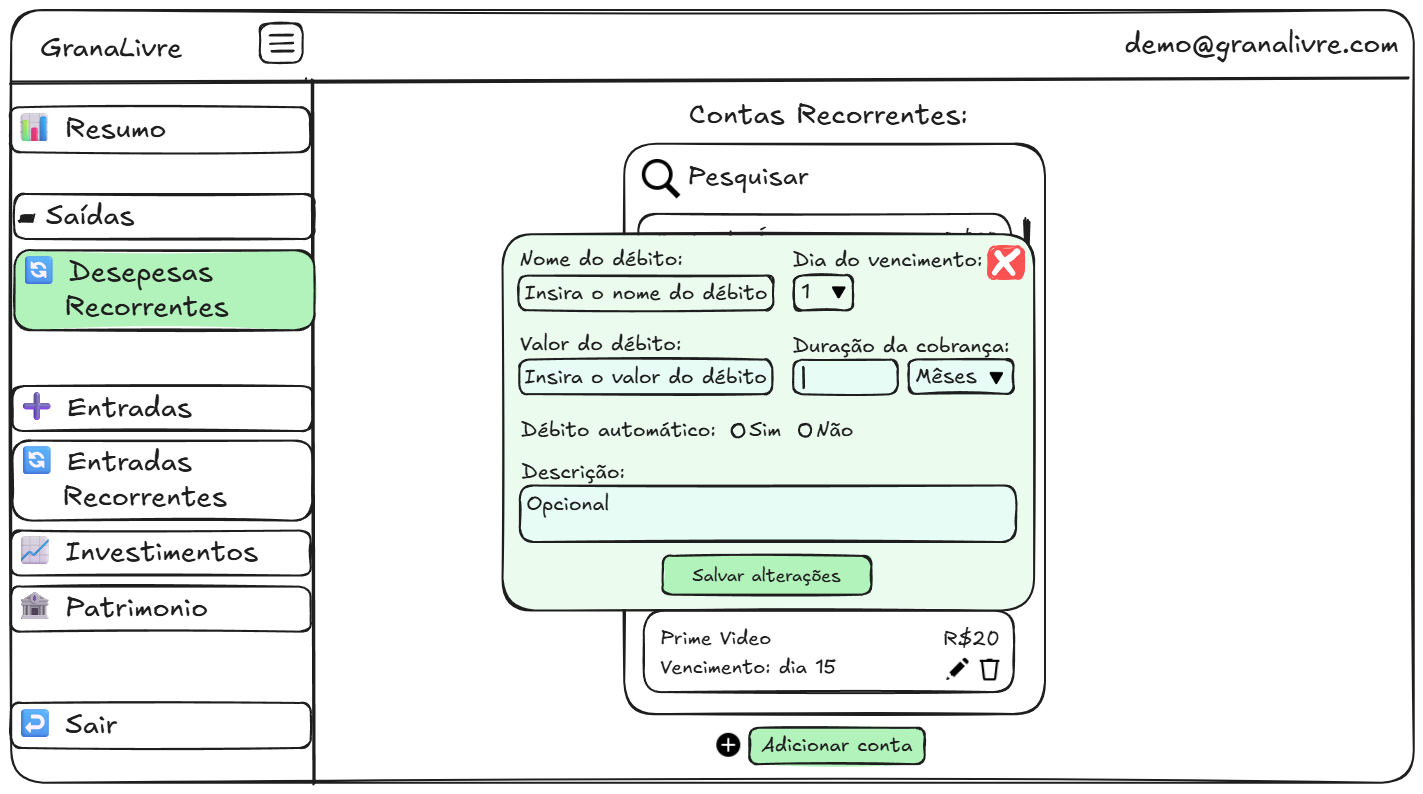
\includegraphics[width=0.9\textwidth]{imgs/04-despesas_recorrentes_1.png}
    \caption{Protótipo de baixa fidelidade da tela de gerenciamento de despesas recorrentes com formulário para adicionar nova despesa}
    \label{fig:prot_despesas_recorrentes1}
\end{figure}

\begin{figure}[H]
    \centering
    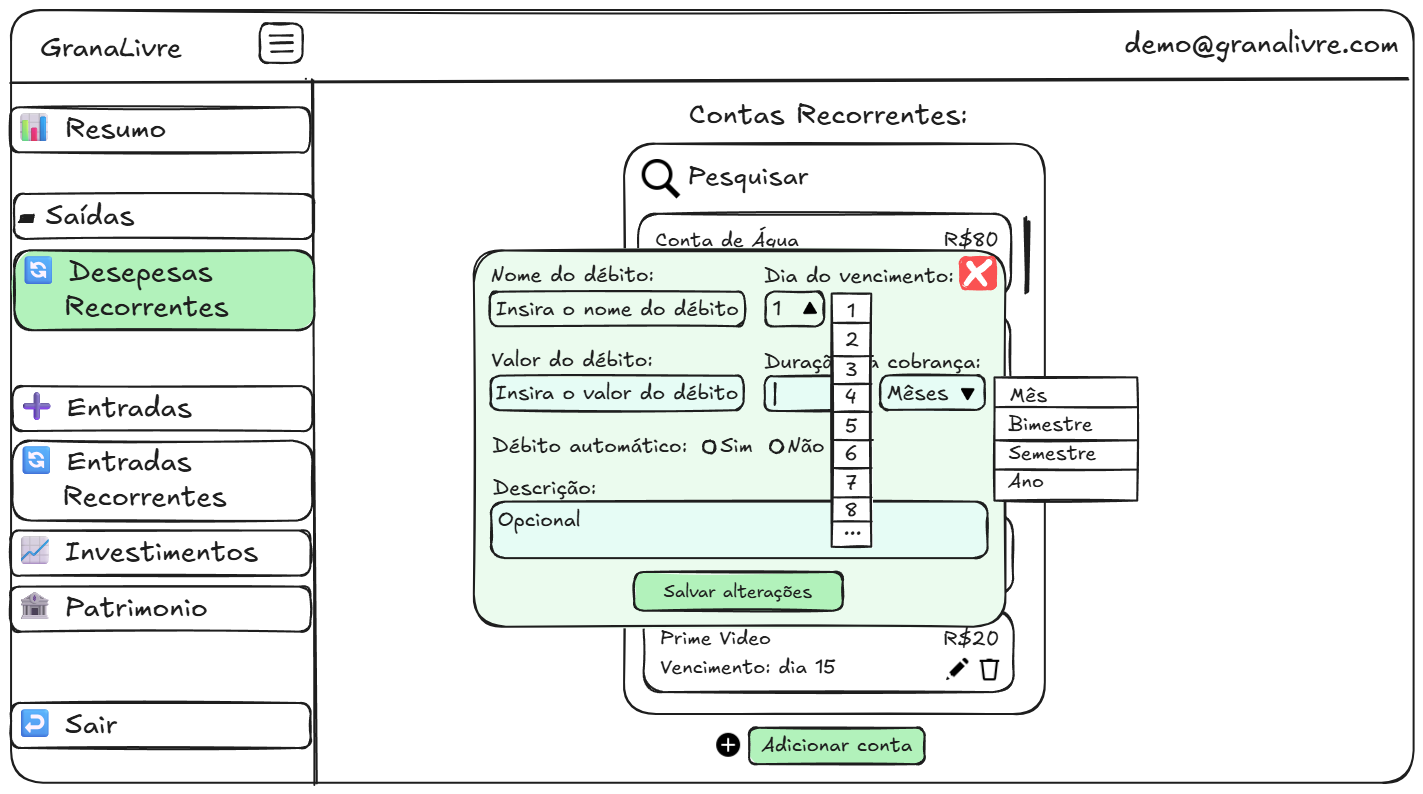
\includegraphics[width=0.9\textwidth]{imgs/04-despesas_recorrentes_2.png}
    caption{Protótipo de baixa fidelidade da tela de gerenciamento de despesas recorrentes com menus dropdown ao adicionar nova despesa}
    \label{fig:prot_despesas_recorrentes2}
\end{figure}

\begin{figure}[H]
    \centering
    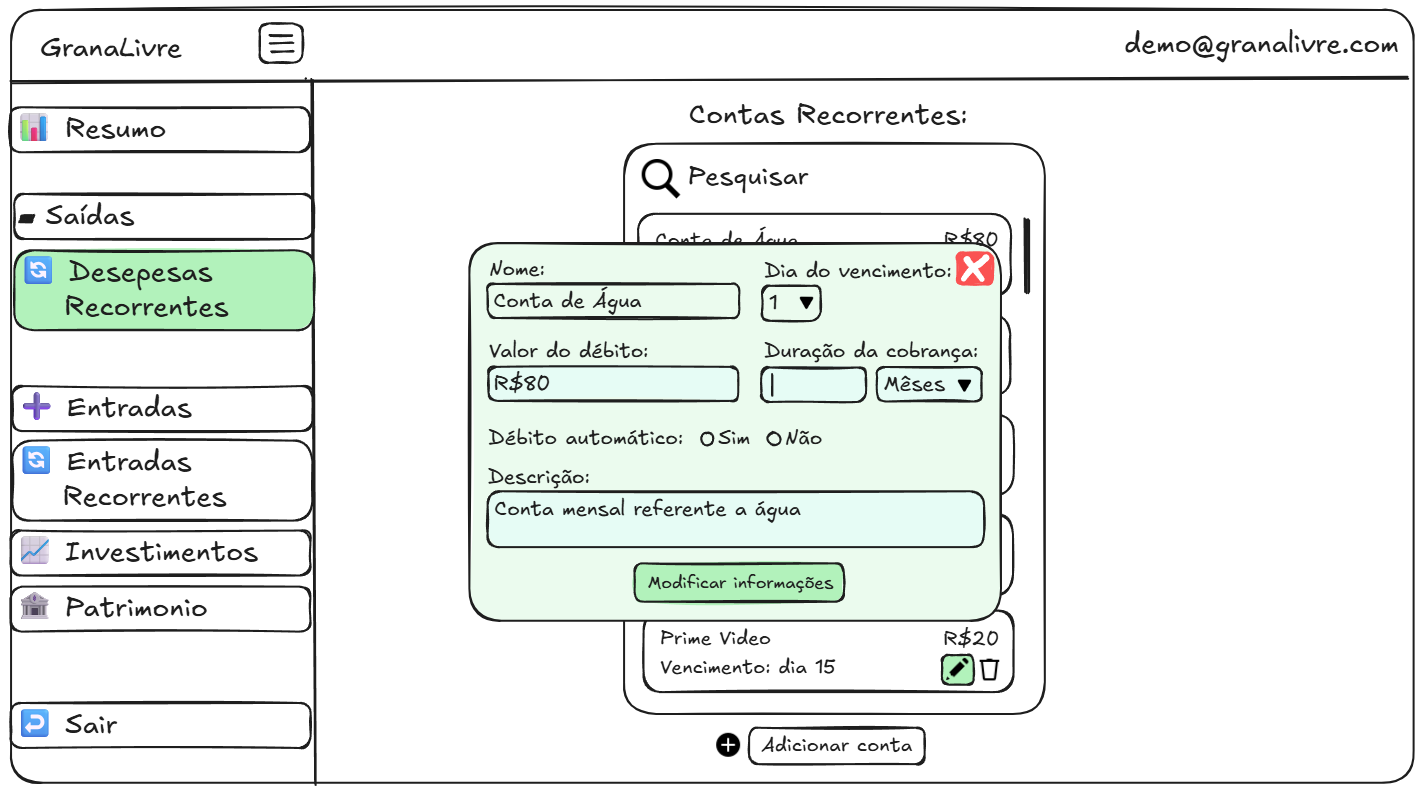
\includegraphics[width=0.9\textwidth]{imgs/04-despesas_recorrentes_3.png}
    \caption{Protótipo de baixa fidelidade da tela de gerenciamento de despesas recorrentes com formulário para editar uma despesa existente}
    \label{fig:prot_despesas_recorrentes3}
\end{figure}

\begin{figure}[H]
    \centering
    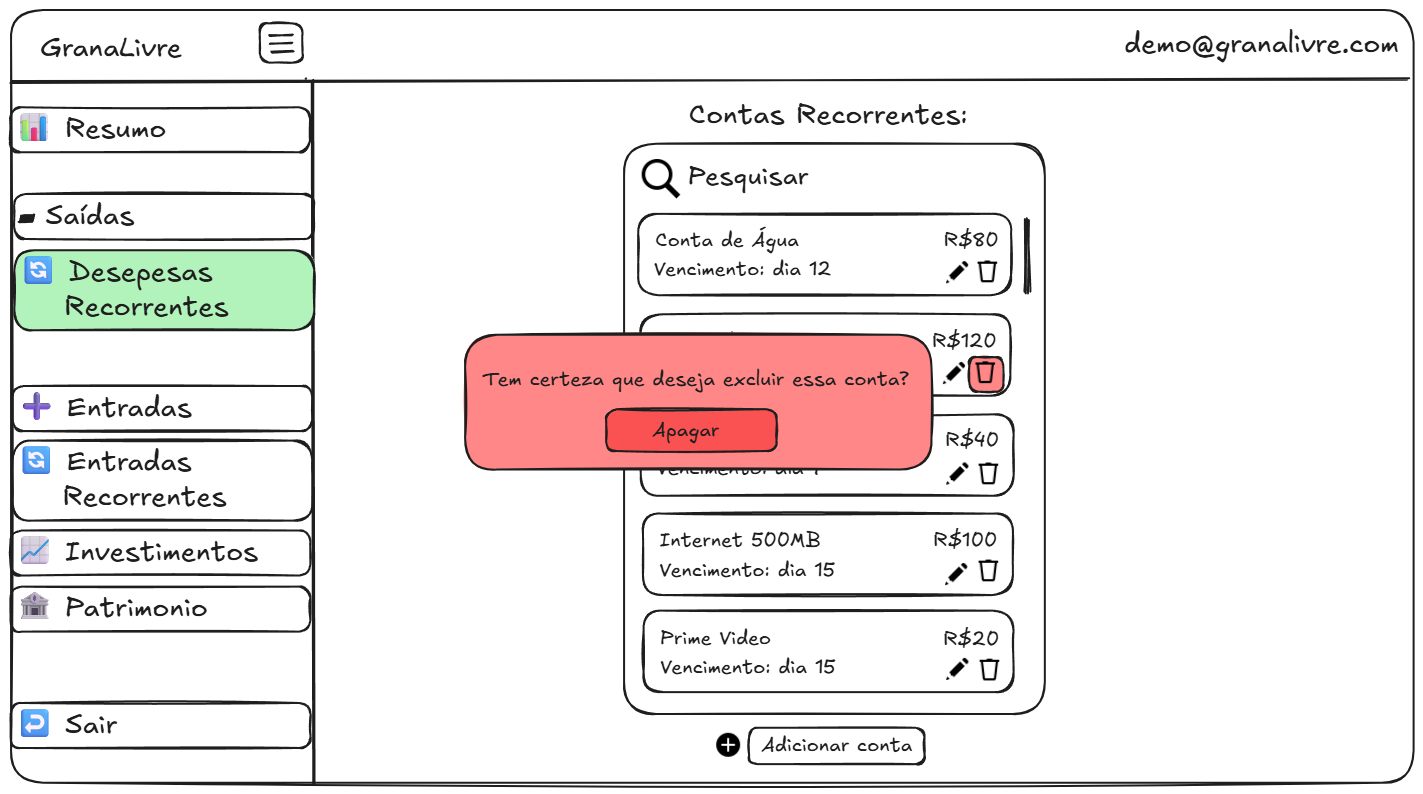
\includegraphics[width=0.9\textwidth]{imgs/04-despesas_recorrentes_4.png}
    \caption{Protótipo de baixa fidelidade da tela de gerenciamento de despesas recorrentes com opção de exclusão de uma despesa existente}
    \label{fig:prot_despesas_recorrentes4}
\end{figure}

%05-saidas.png até 05-saidas5.png
\begin{figure}[H]
    \centering
    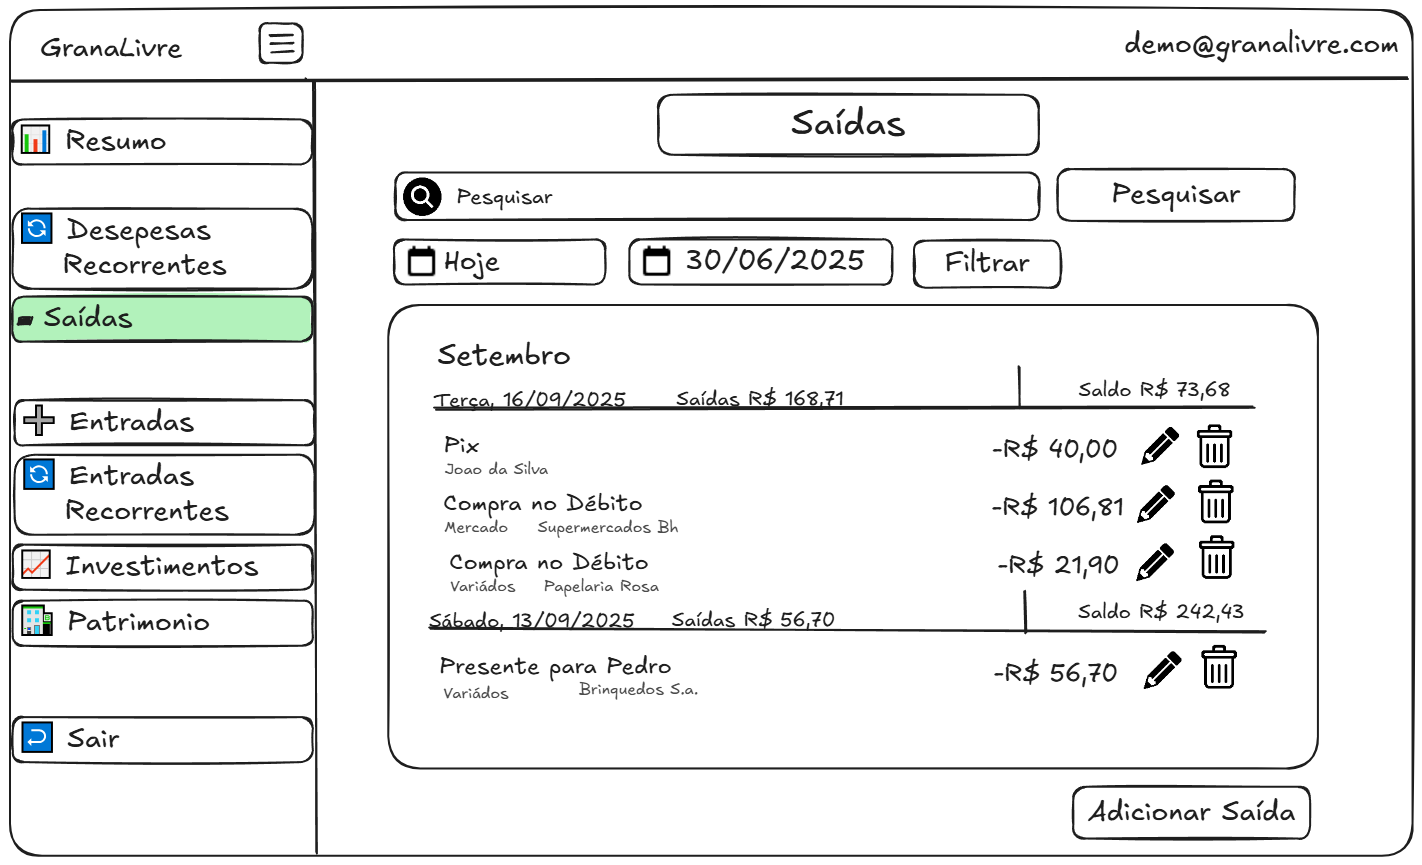
\includegraphics[width=0.9\textwidth]{imgs/05-saidas.png}
    \caption{Protótipo de baixa fidelidade da tela de gerenciamento de saídas}
    \label{fig:prot_saidax}
\end{figure}

\begin{figure}[H]
    \centering
    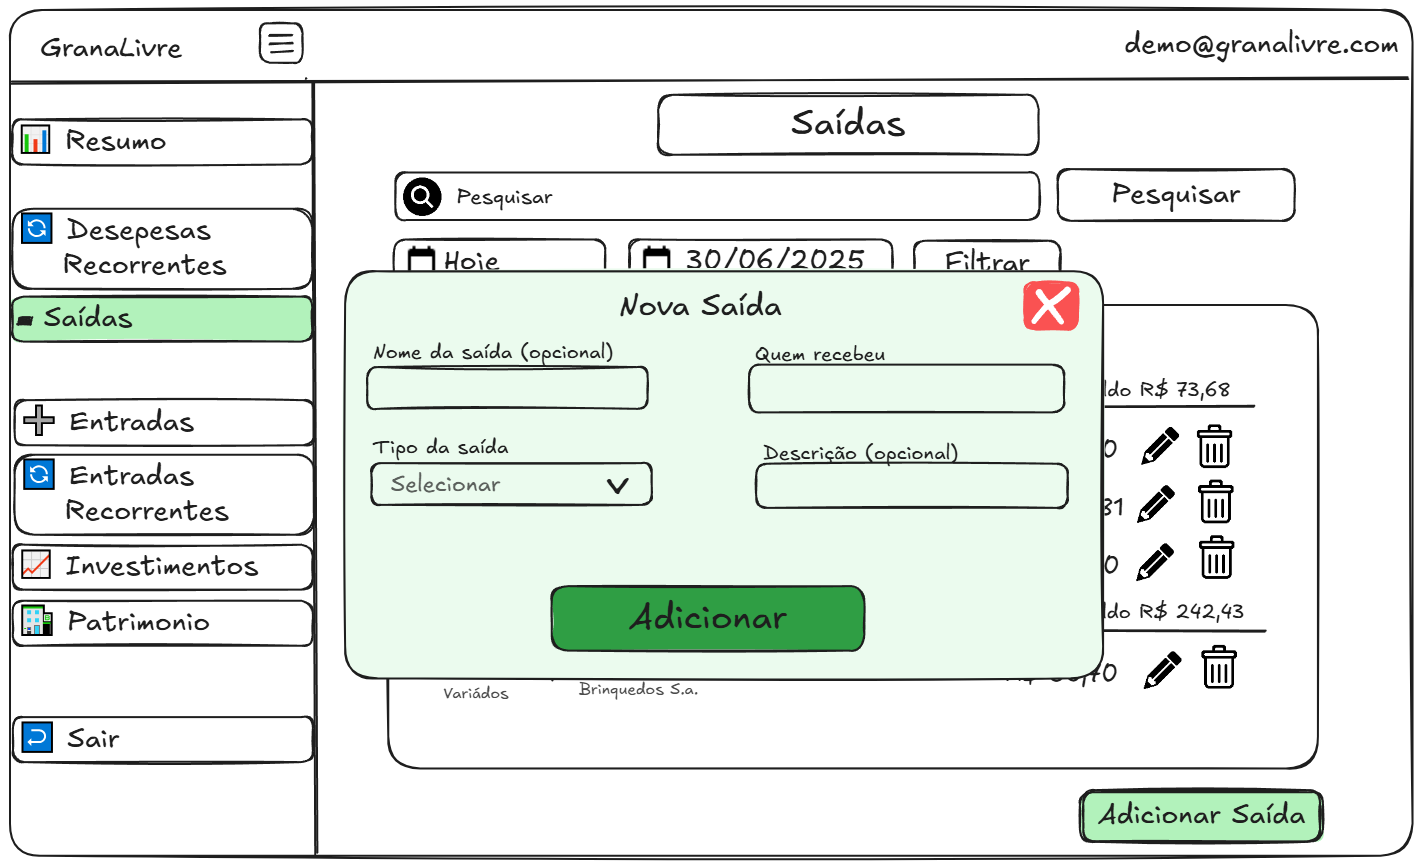
\includegraphics[width=0.9\textwidth]{imgs/05-saidas2.png}
    \caption{Protótipo de baixa fidelidade da tela de gerenciamento de saídas com formulário para adicionar nova saída}
    \label{fig:prot_saidax2}
\end{figure}

\begin{figure}[H]
    \centering
    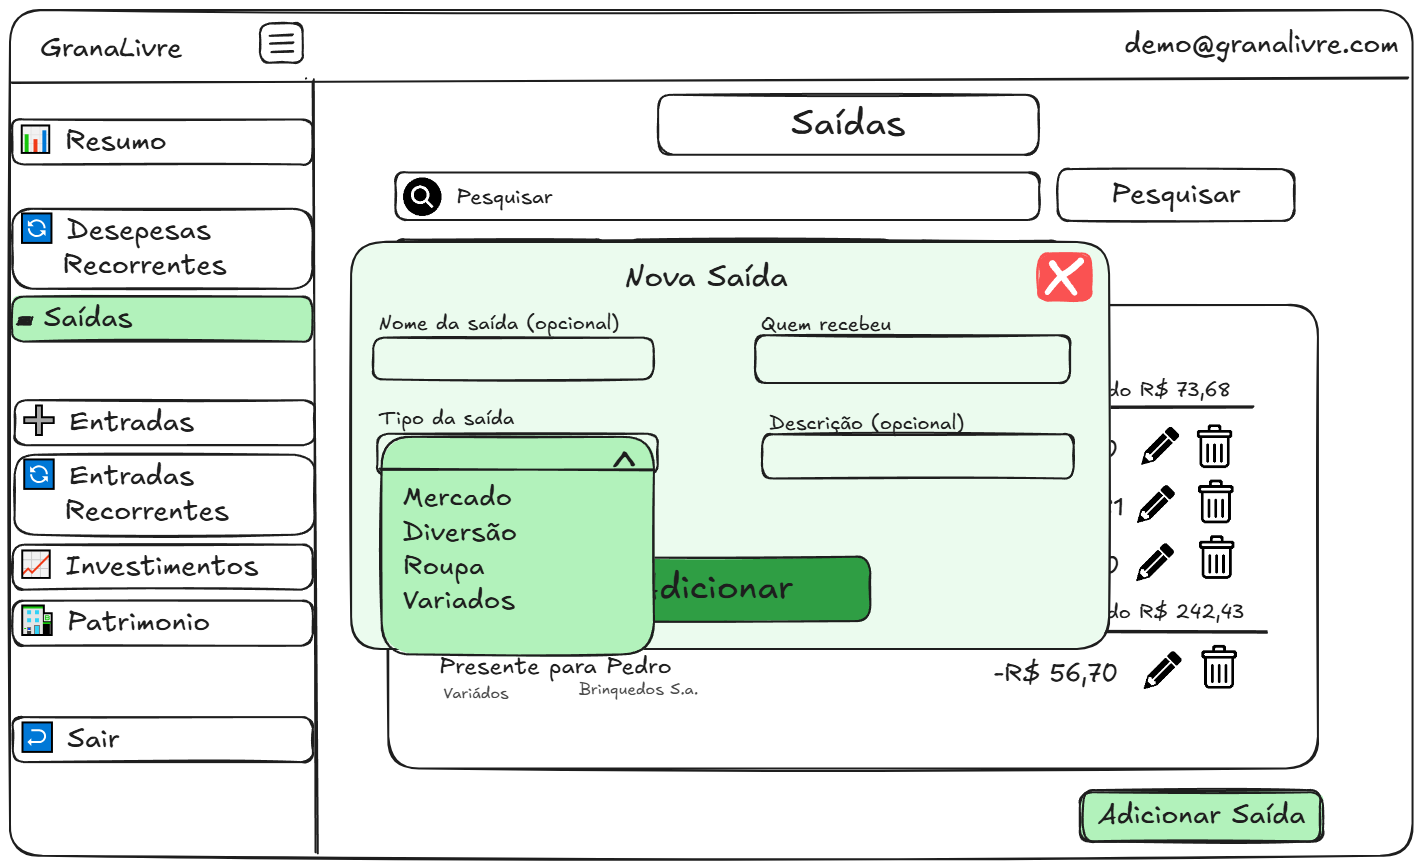
\includegraphics[width=0.9\textwidth]{imgs/05-saidas3.png}
    \caption{Protótipo de baixa fidelidade da tela de gerenciamento de saídas com menus dropdown ao adicionar nova saída}
    \label{fig:prot_saidax3}
\end{figure}

\begin{figure}[H]
    \centering
    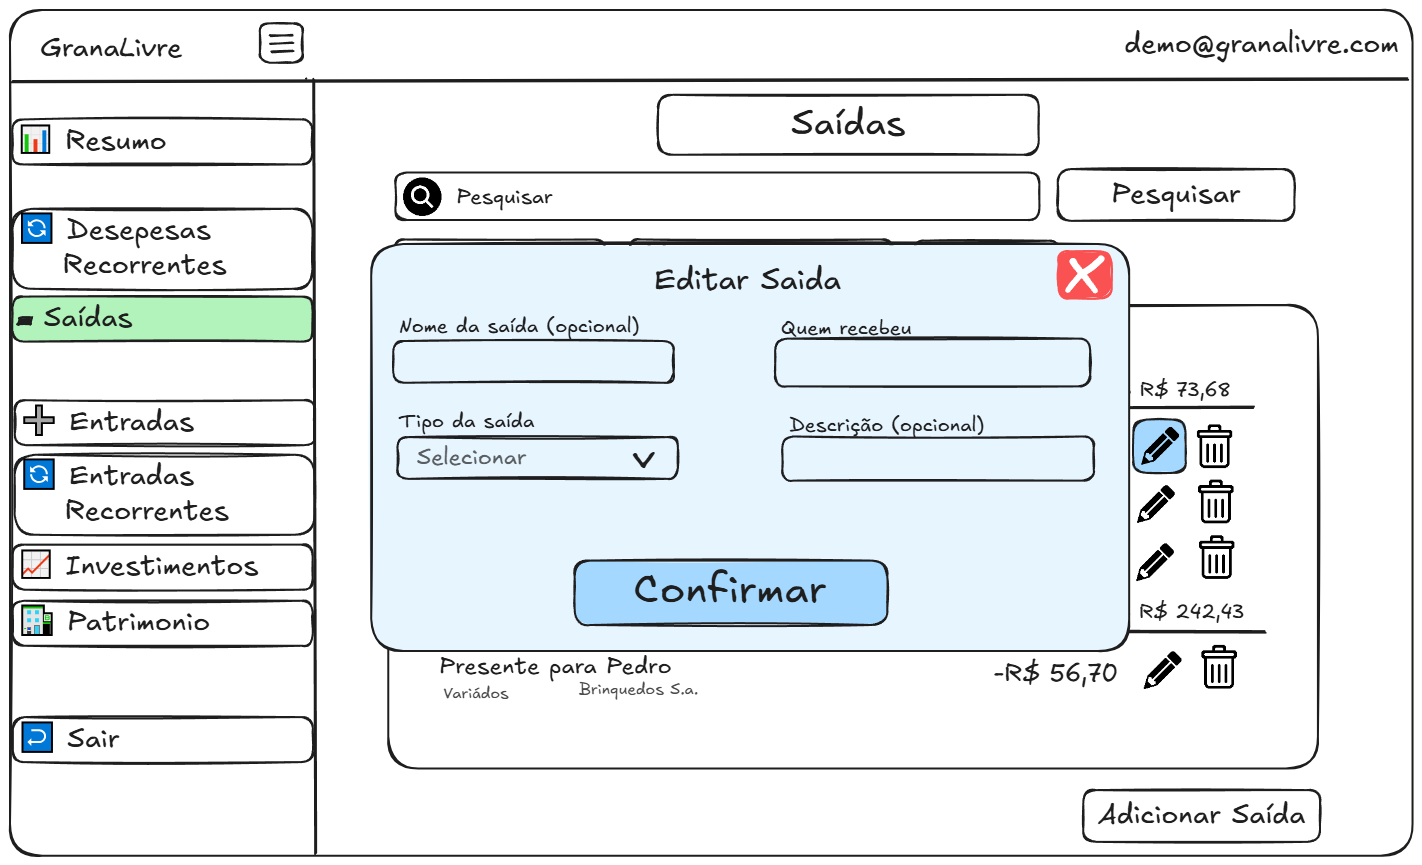
\includegraphics[width=0.9\textwidth]{imgs/05-saidas4.png}
    \caption{Protótipo de baixa fidelidade da tela de gerenciamento de saídas com formulário para editar uma saída existente}
    \label{fig:prot_saidax4}
\end{figure}

\begin{figure}[H]
    \centering
    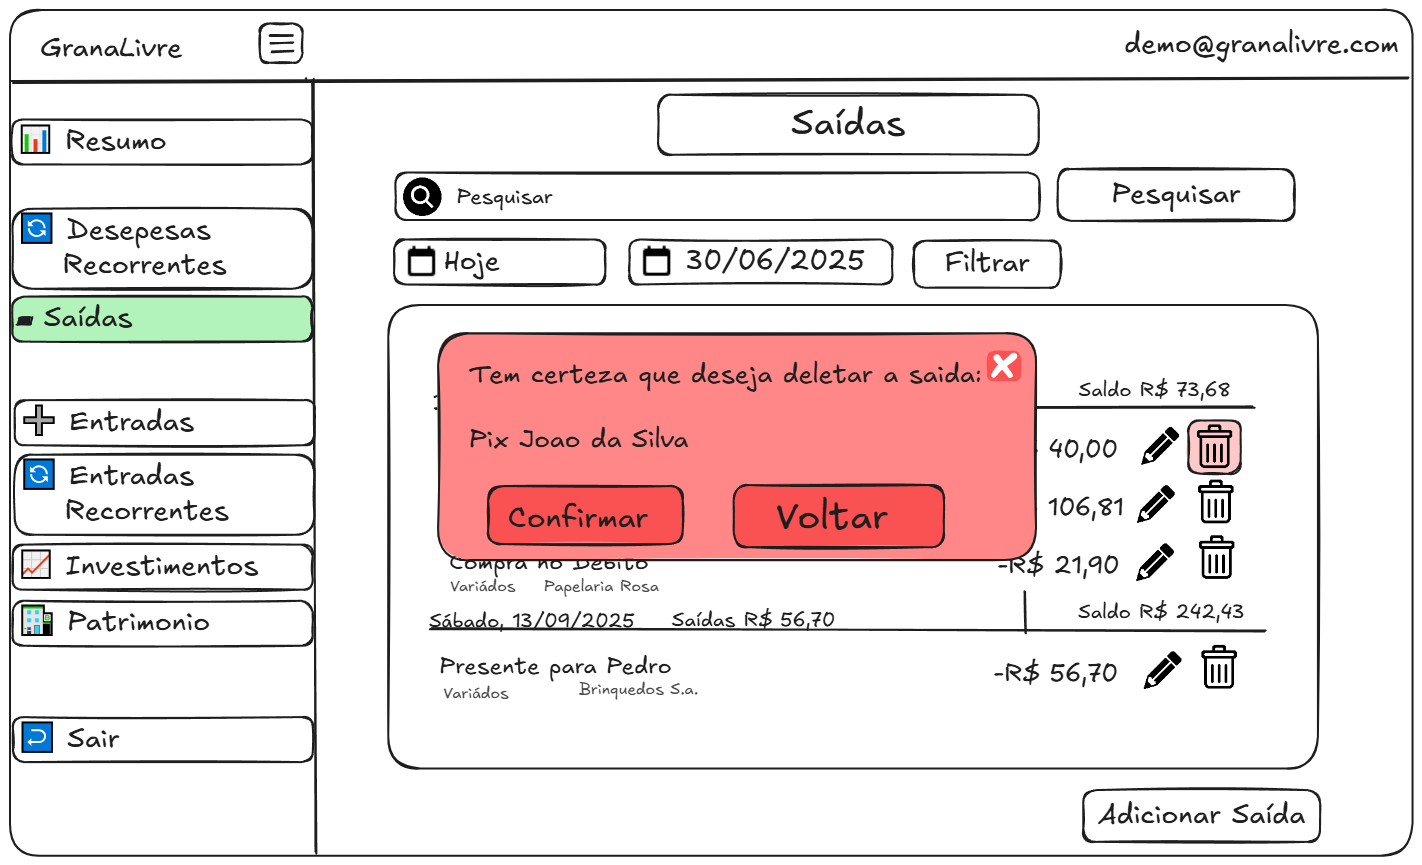
\includegraphics[width=0.9\textwidth]{imgs/05-saidas5.png}
    \caption{Protótipo de baixa fidelidade da tela de gerenciamento de saídas com confirmação para exclusão de uma saída}
    \label{fig:prot_saidax5}
\end{figure}

%06-entradas.png até 06-entradas5.png
\begin{figure}[H]
    \centering
    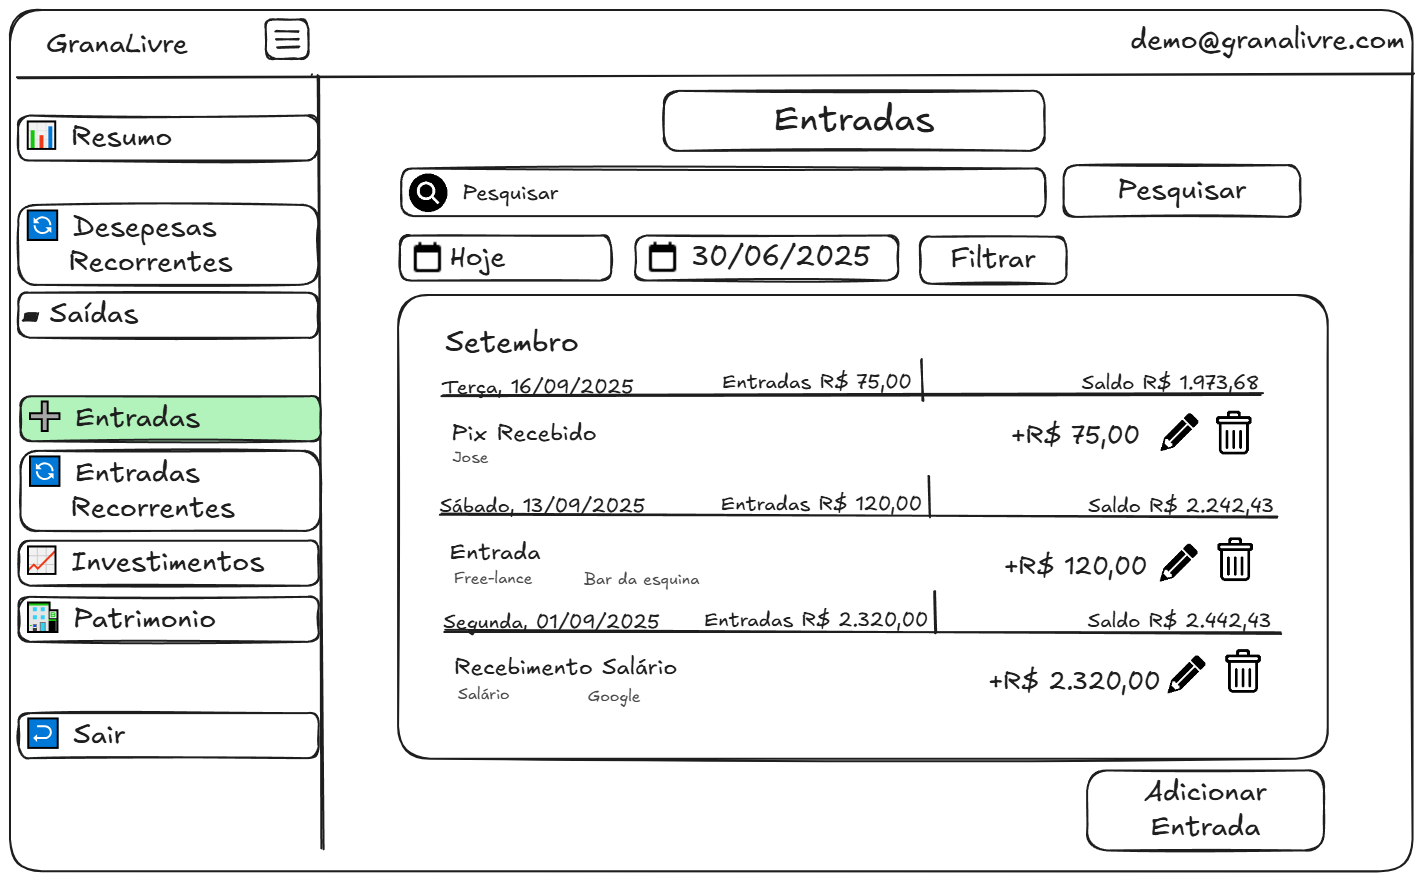
\includegraphics[width=0.9\textwidth]{imgs/06-entradas.png}
    \caption{Protótipo de baixa fidelidade da tela de gerenciamento de entradas}
    \label{fig:prot_entradas}
\end{figure}

\begin{figure}[H]
    \centering
    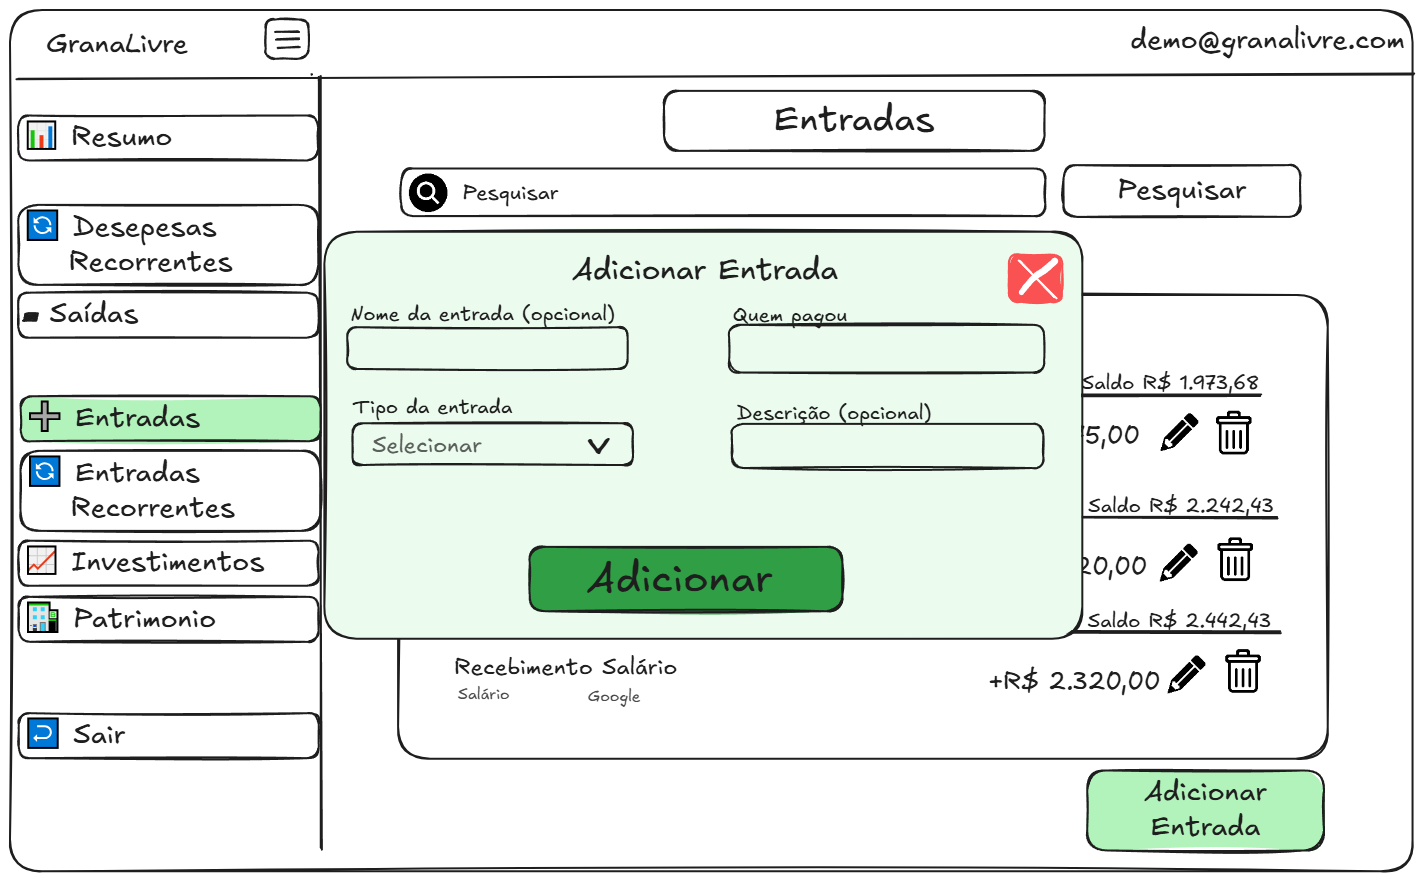
\includegraphics[width=0.9\textwidth]{imgs/06-entradas2.png}
    \caption{Protótipo de baixa fidelidade da tela de gerenciamento de entradas com formulário para adicionar nova entrada}
    \label{fig:prot_entradas2}
\end{figure}

\begin{figure}[H]
    \centering
    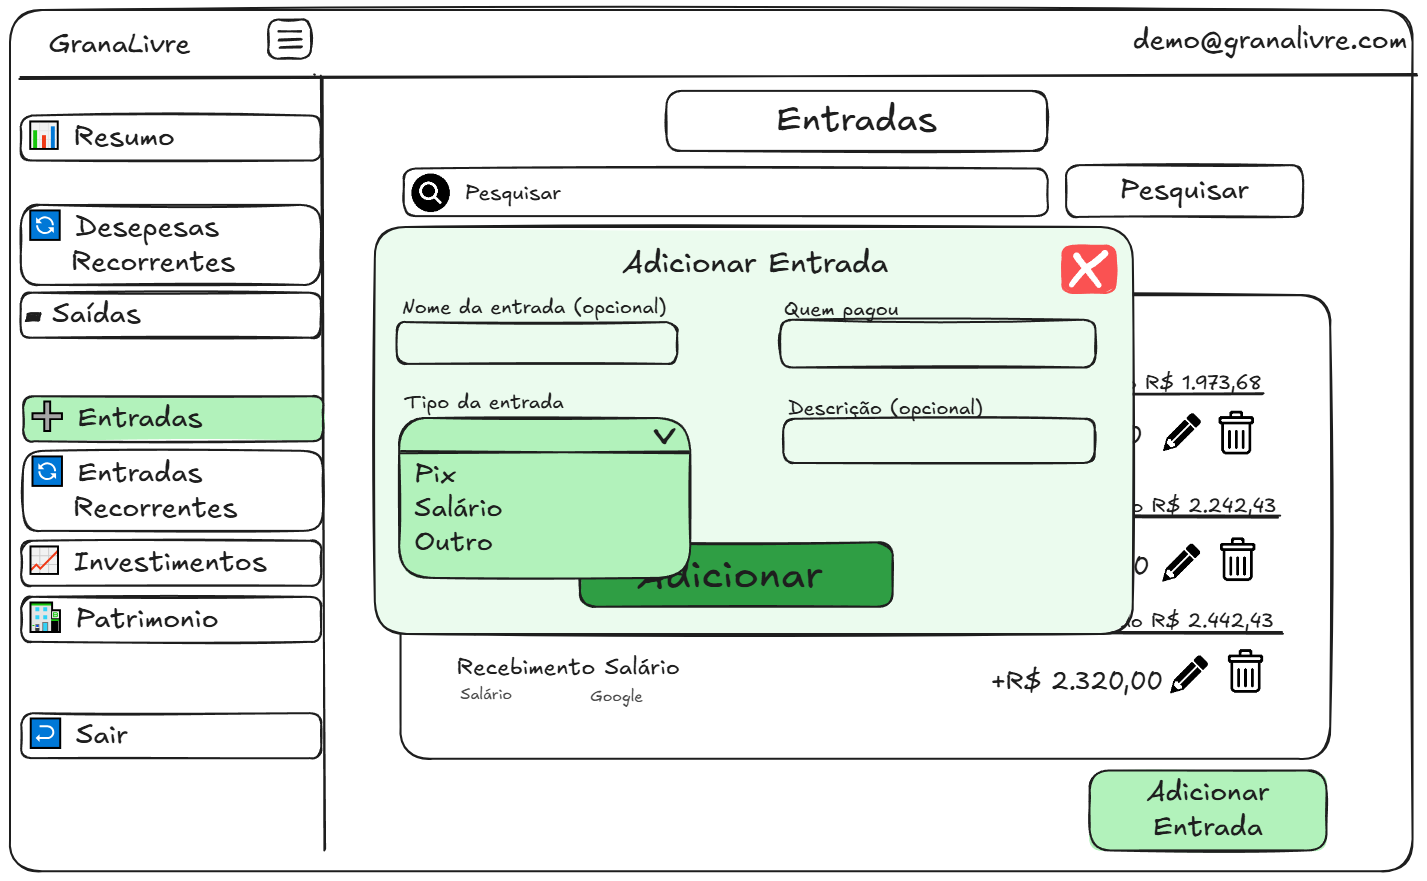
\includegraphics[width=0.9\textwidth]{imgs/06-entradas3.png}
    \caption{Protótipo de baixa fidelidade da tela de gerenciamento de entradas com menus dropdown ao adicionar nova entrada}
    \label{fig:prot_entradas3}
\end{figure}

\begin{figure}[H]
    \centering
    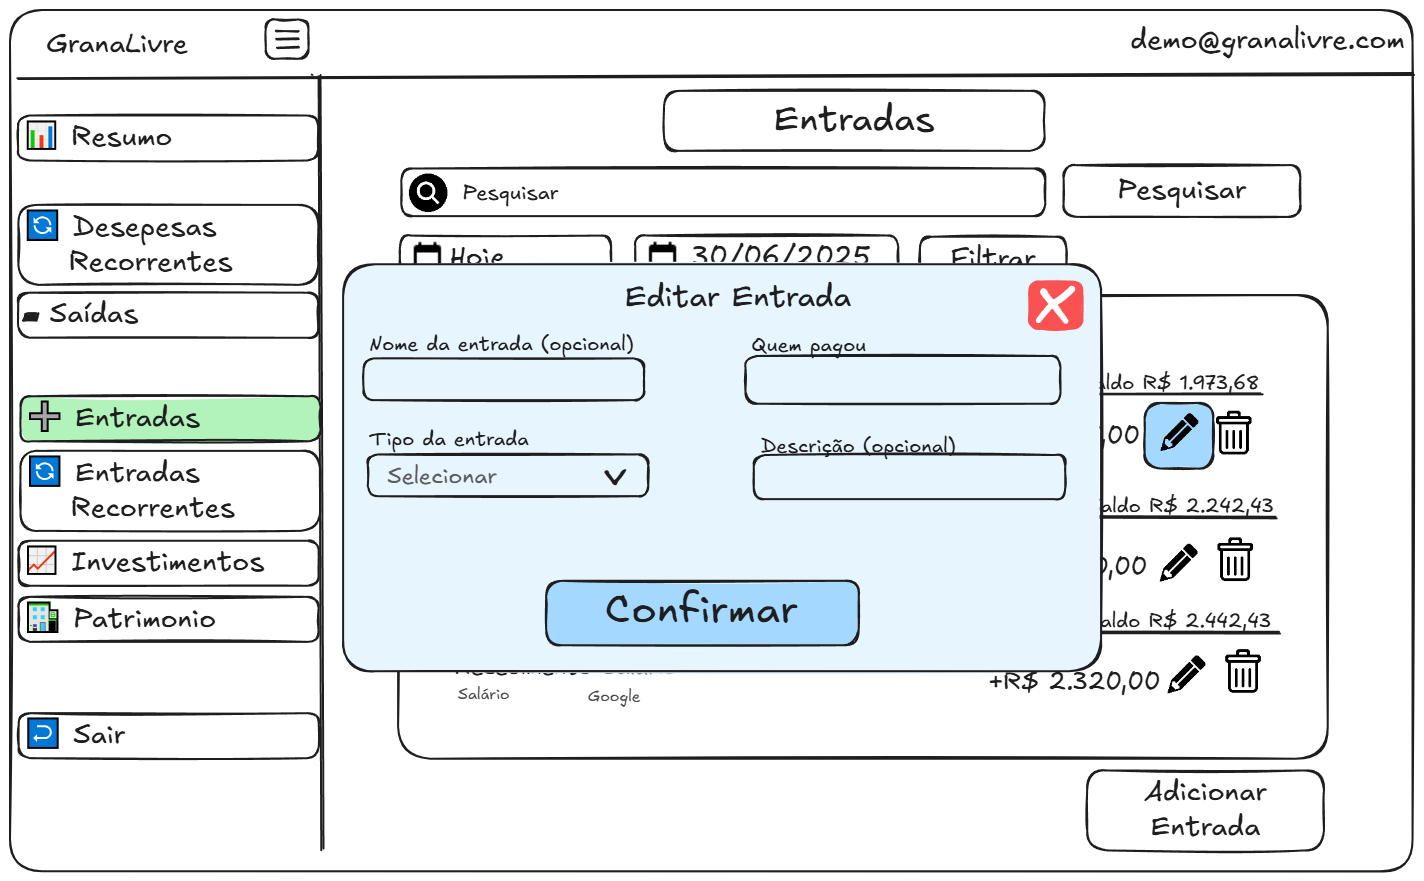
\includegraphics[width=0.9\textwidth]{imgs/06-entradas4.png}
    \caption{Protótipo de baixa fidelidade da tela de gerenciamento de entradas com formulário para editar uma entrada existente}
    \label{fig:prot_entradas4}
\end{figure}

\begin{figure}[H]
    \centering
    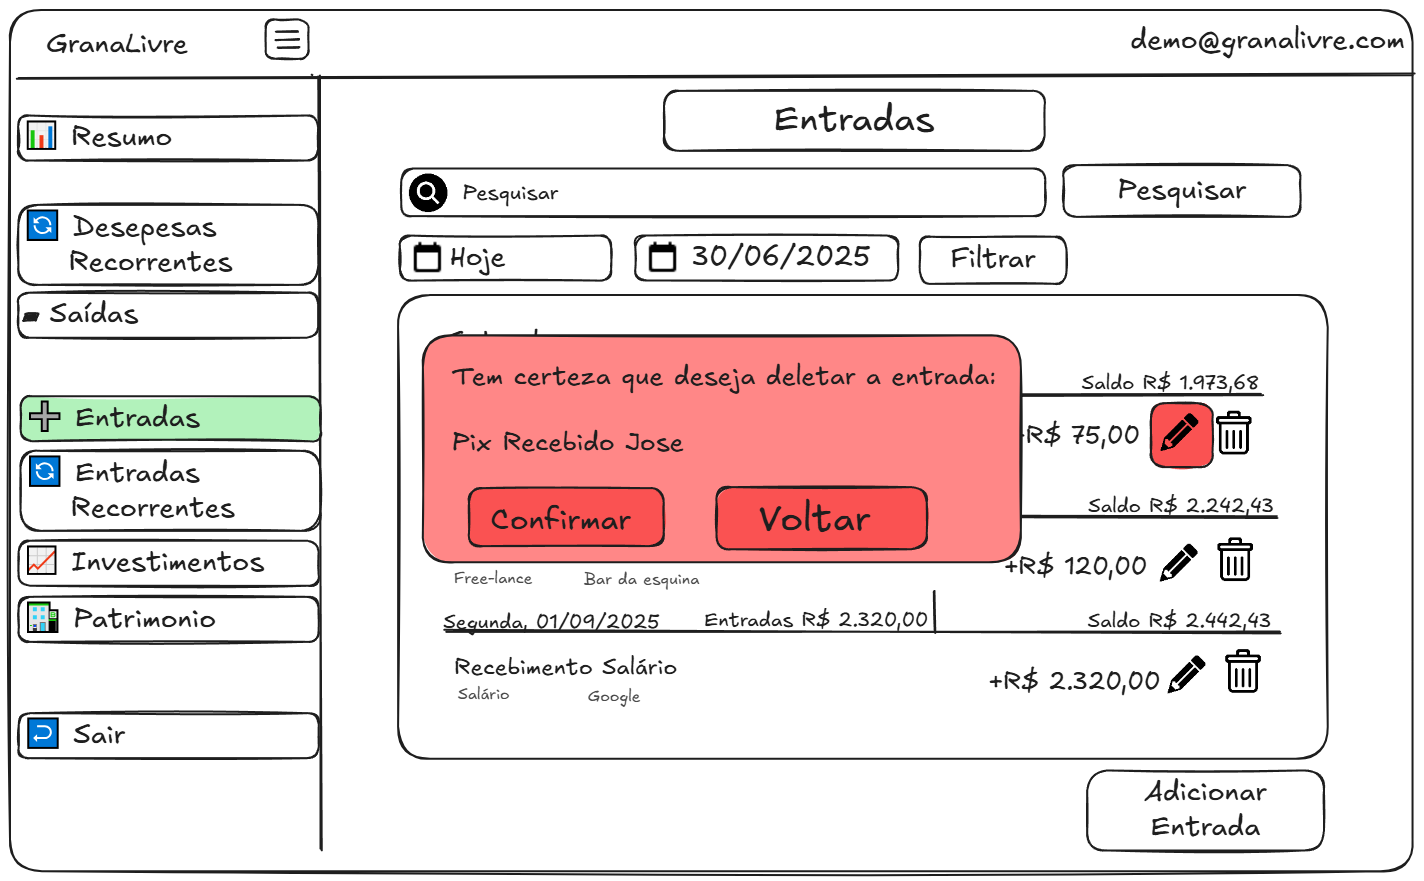
\includegraphics[width=0.9\textwidth]{imgs/06-entradas5.png}
    \caption{Protótipo de baixa fidelidade da tela de gerenciamento de entradas com confirmação para exclusão de uma entrada}
    \label{fig:prot_entradas5}
\end{figure}

%07-entradas-recorrentes.png
\begin{figure}[H]
    \centering
    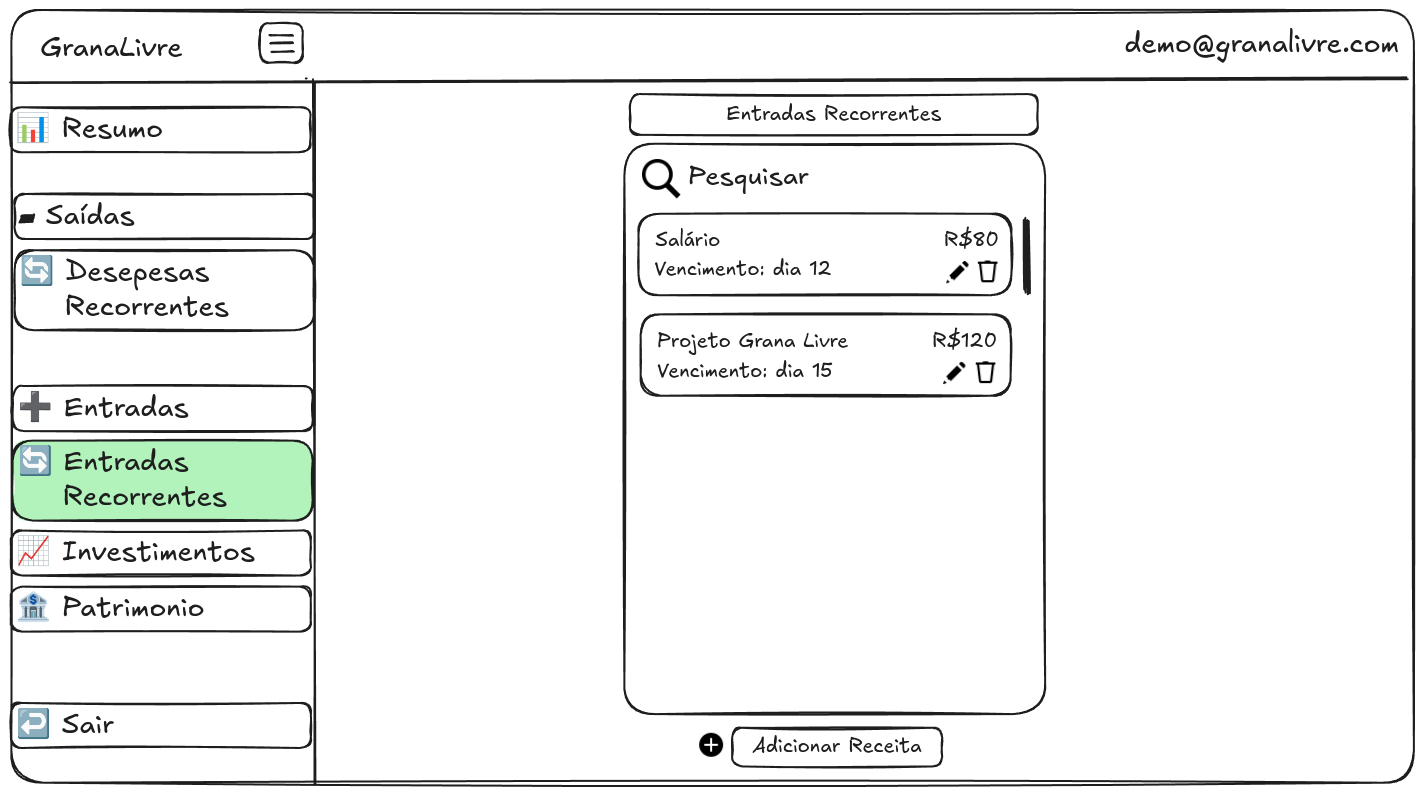
\includegraphics[width=0.9\textwidth]{imgs/07-entradas-recorrentes.png}
    \caption{Protótipo de baixa fidelidade da tela de gerenciamento de entradas recorrentes}
    \label{fig:prot_entradas_recorrentes}
\end{figure}

%07-entradas-recorrentes2.png adicionando nova entrada recorrente
\begin{figure}[H]
    \centering
    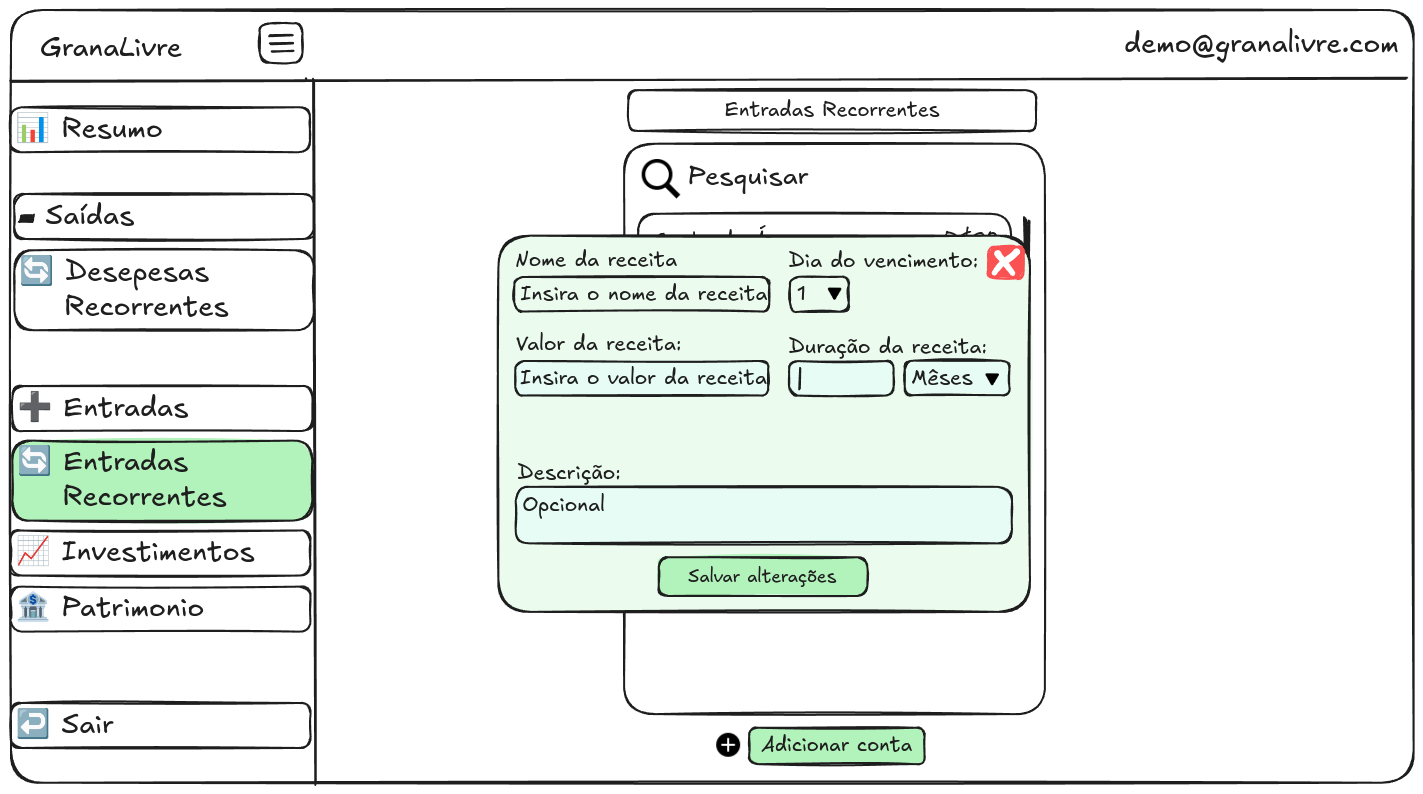
\includegraphics[width=0.9\textwidth]{imgs/07-entradas-recorrentes2.png}
    \caption{Protótipo de baixa fidelidade da tela de gerenciamento de entradas recorrentes com formulário para adicionar nova entrada}
    \label{fig:prot_entradas_recorrentes2}
\end{figure}

%07-entradas-recorrentes3.png mostrando menus com dropdown ao adicionar nova entrada recorrente
\begin{figure}[H]
    \centering
    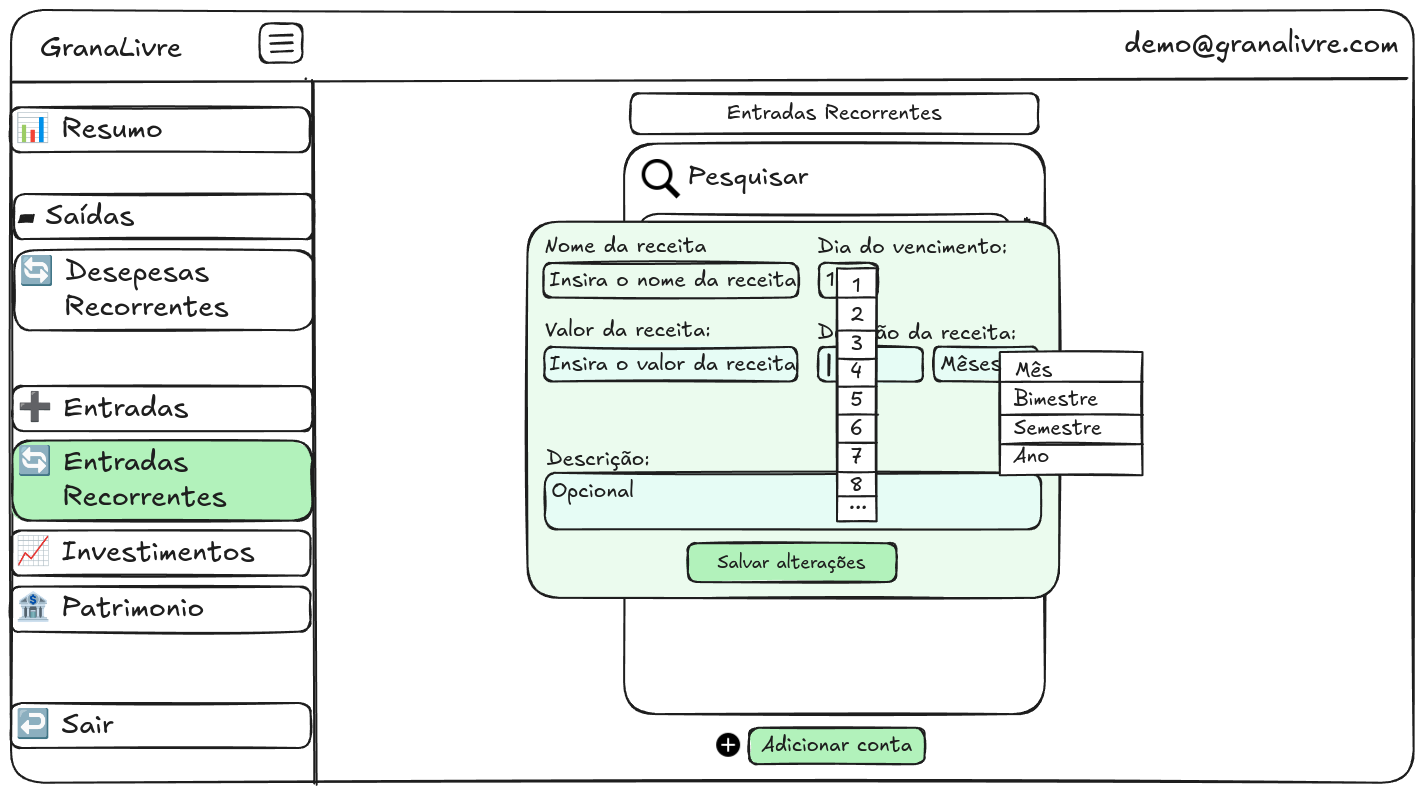
\includegraphics[width=0.9\textwidth]{imgs/07-entradas-recorrentes3.png}
    \caption{Protótipo de baixa fidelidade da tela de gerenciamento de entradas recorrentes com menus dropdown ao adicionar nova entrada}
    \label{fig:prot_entradas_recorrentes3}
\end{figure}

%07-entradas-recorrentes4.png mostrando tela de edição de entrada recorrente
\begin{figure}[H]
    \centering
    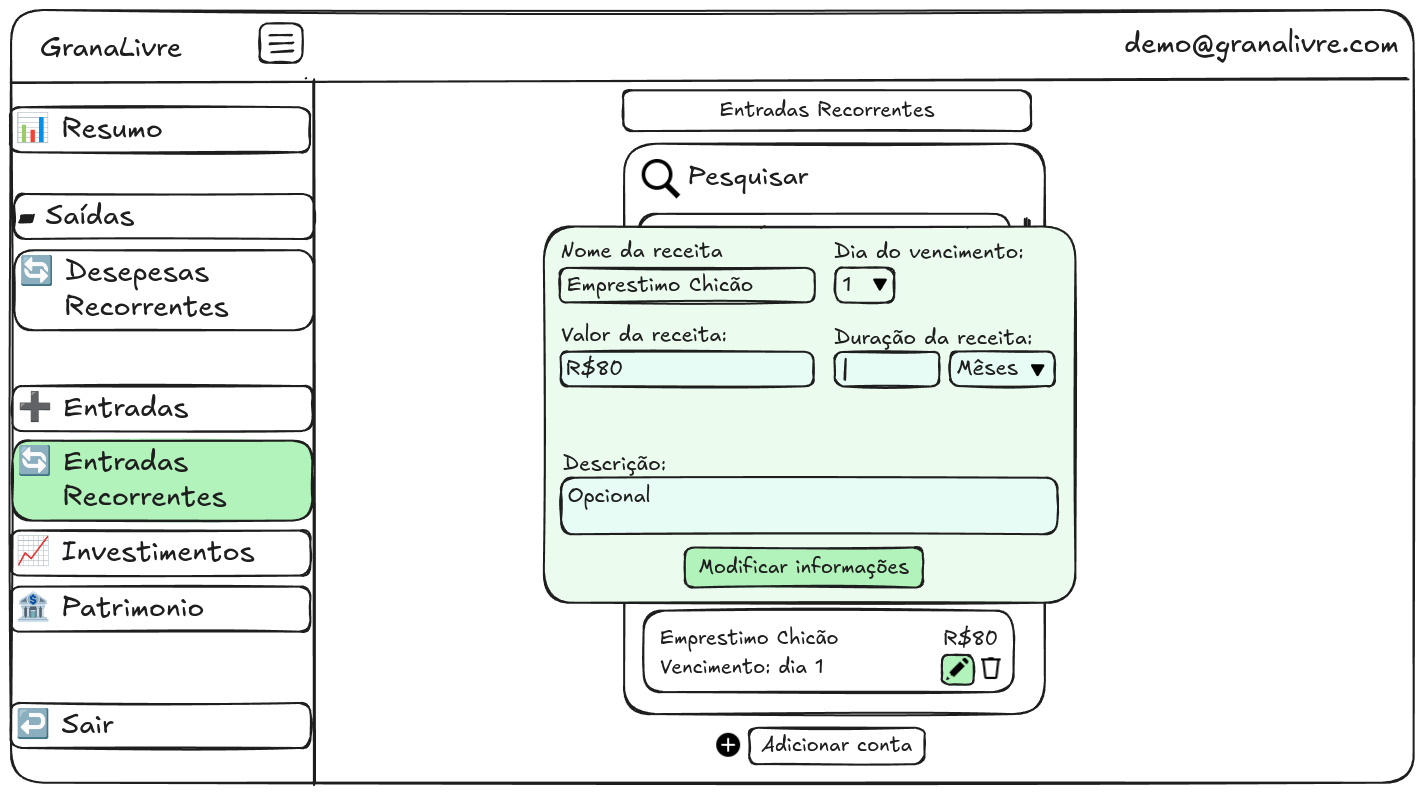
\includegraphics[width=0.9\textwidth]{imgs/07-entradas-recorrentes4.png}
    \caption{Protótipo de baixa fidelidade da tela de gerenciamento de entradas recorrentes com formulário para editar uma entrada existente}
    \label{fig:prot_entradas_recorrentes4}
\end{figure}

%07-entradas-recorrentes5.png mostrando tela de exclusão de entrada recorrente
\begin{figure}[H]
    \centering
    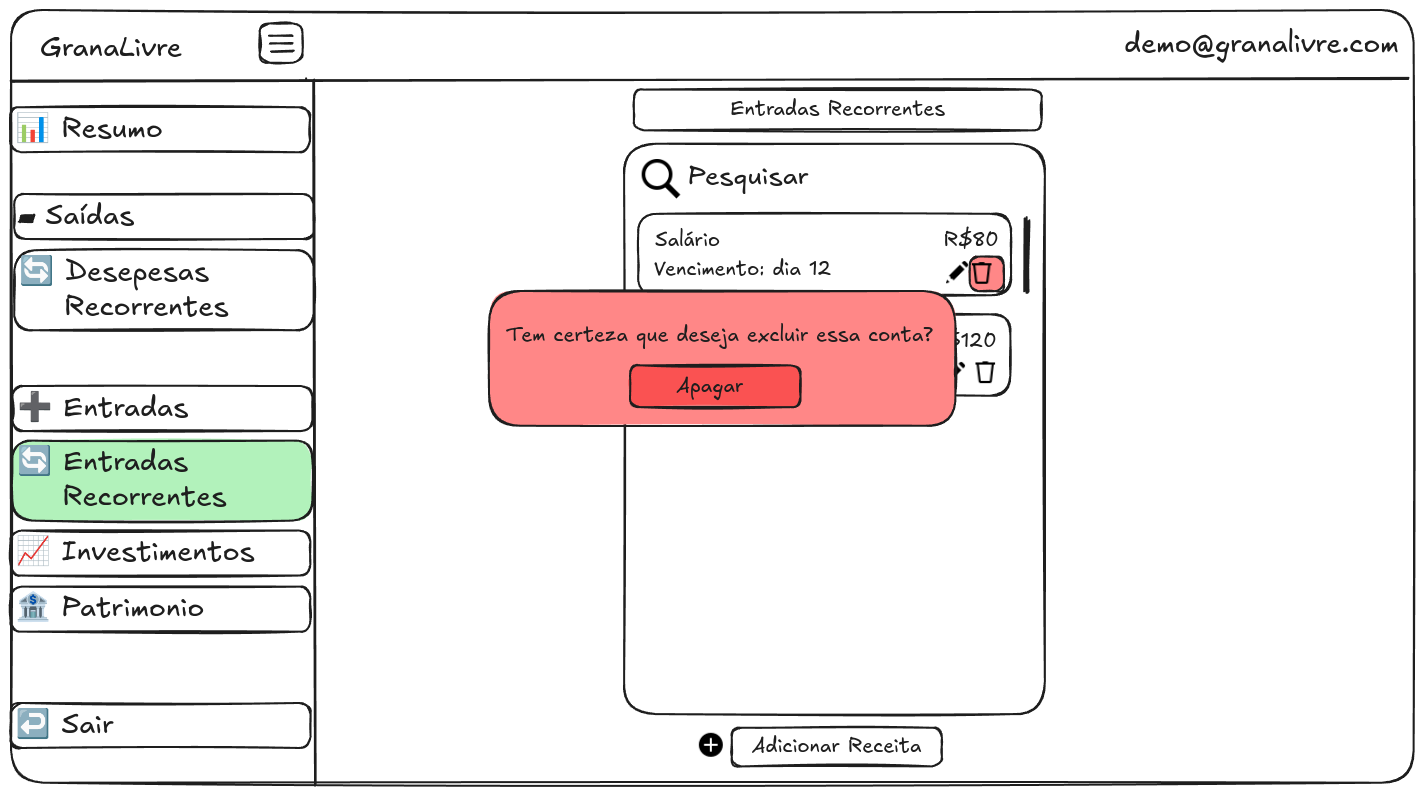
\includegraphics[width=0.9\textwidth]{imgs/07-entradas-recorrentes5.png}
    \caption{Protótipo de baixa fidelidade da tela de gerenciamento de entradas recorrentes com confirmação para exclusão de uma entrada}
    \label{fig:prot_entradas_recorrentes5}
\end{figure}

%08-investimentos.png até 08-investimentos_5.png
\begin{figure}[H]
    \centering
    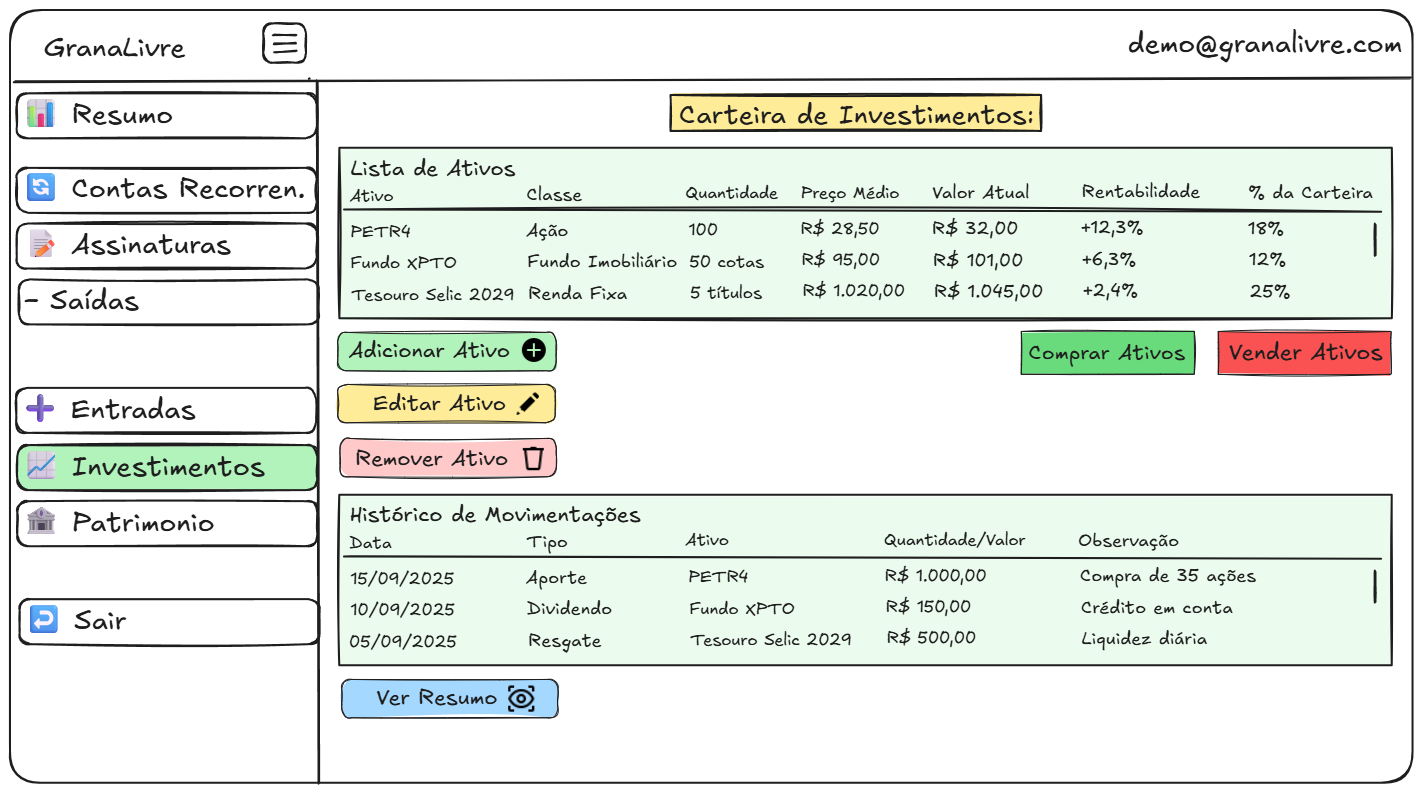
\includegraphics[width=0.9\textwidth]{imgs/08-investimentos.png}
    \caption{Protótipo de baixa fidelidade da tela de gerenciamento de investimentos}
    \label{fig:prot_investimentos}
\end{figure}

\begin{figure}[H]
    \centering
    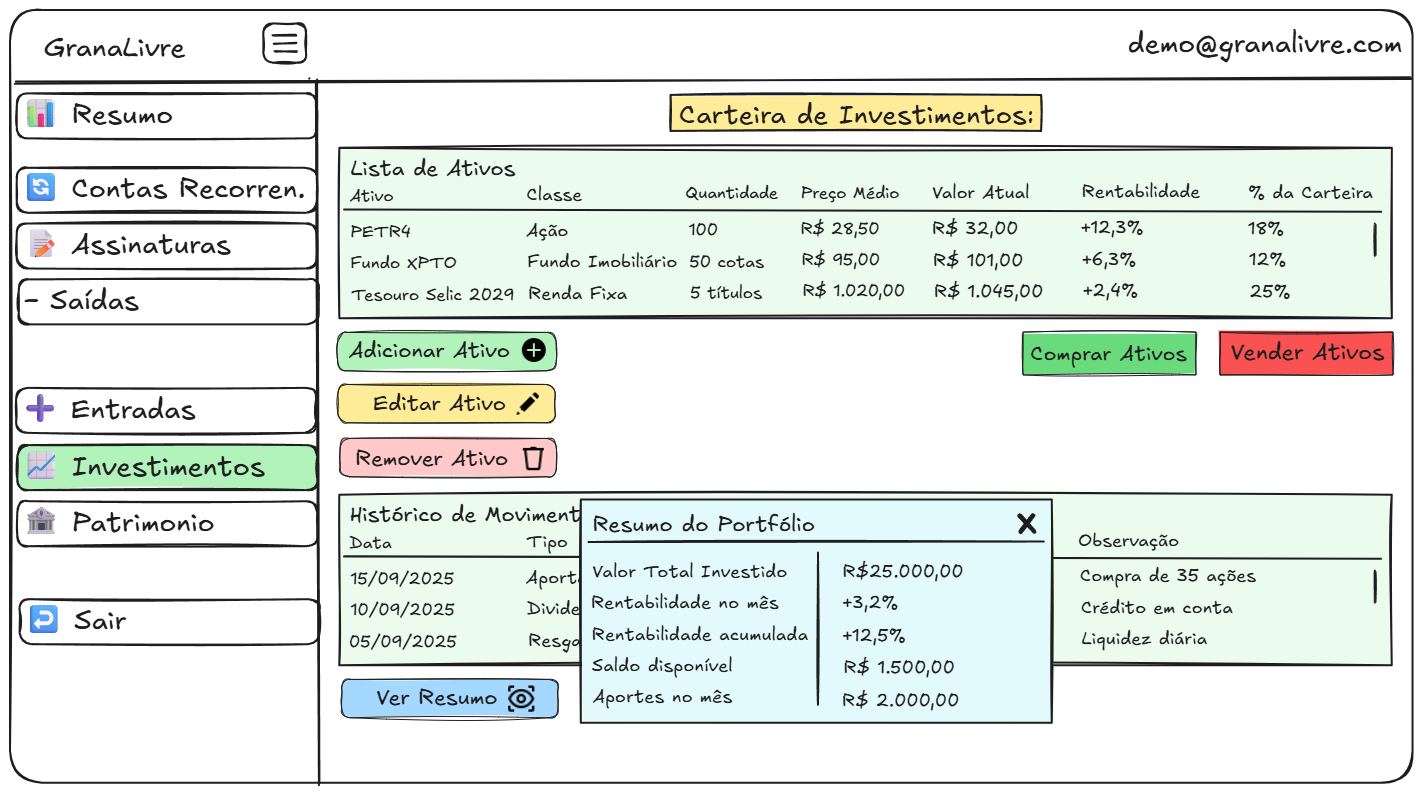
\includegraphics[width=0.9\textwidth]{imgs/08-investimentos_1.png}
    \caption{Protótipo de baixa fidelidade da tela de gerenciamento de investimentos com resumo financeiro}
    \label{fig:prot_investimentos2}
\end{figure}

\begin{figure}[H]
    \centering
    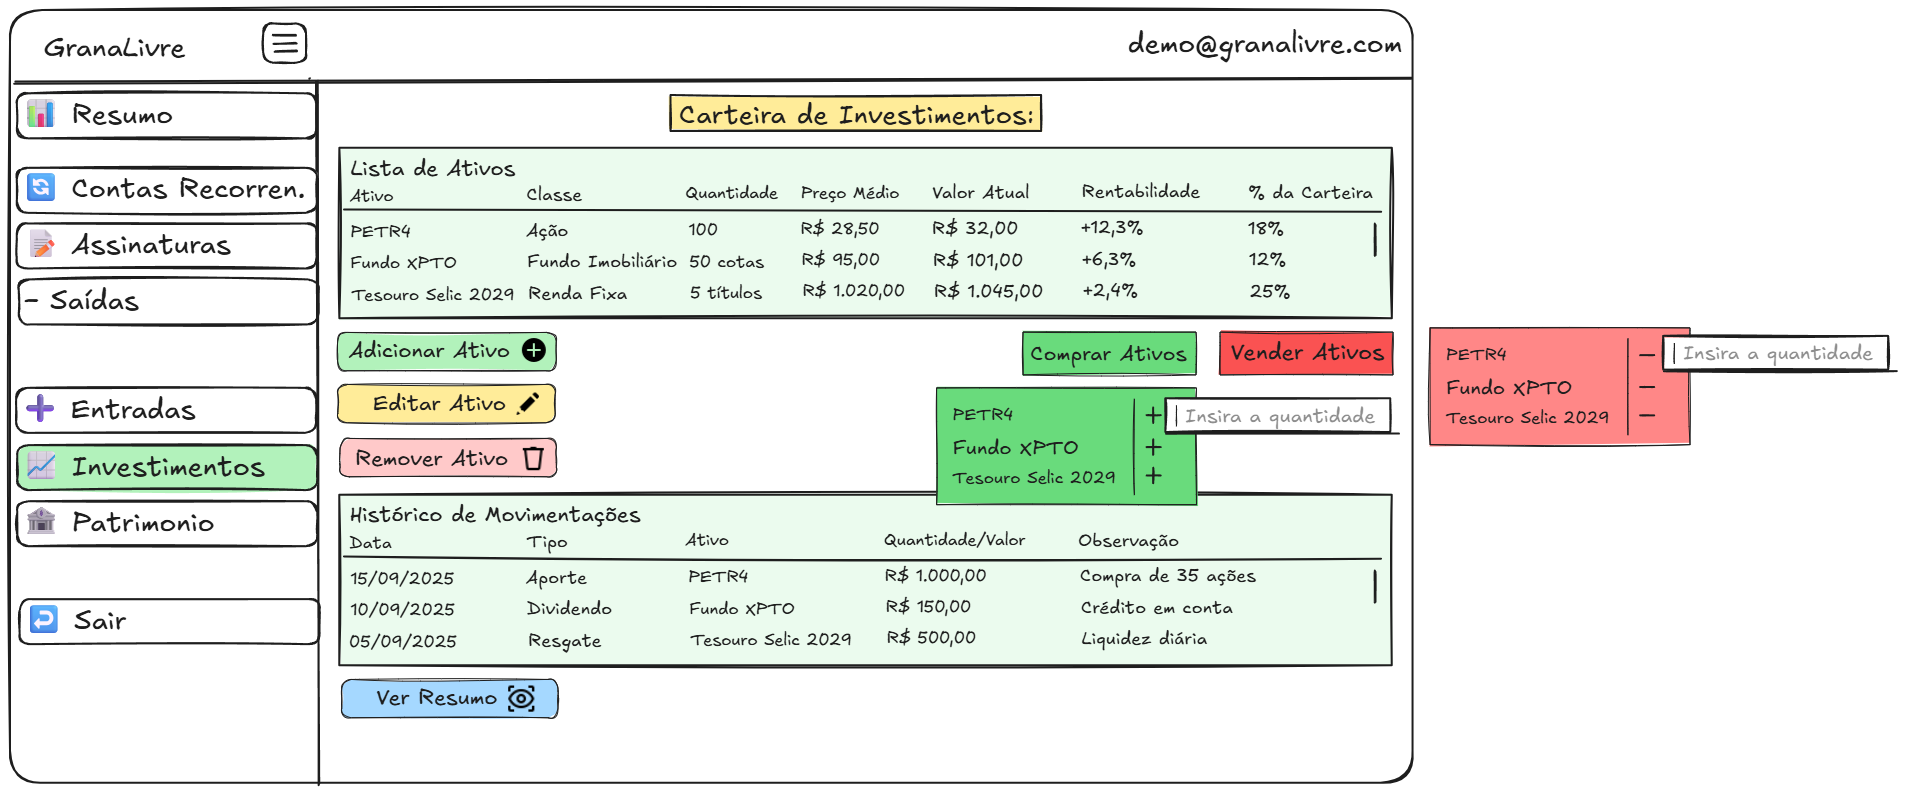
\includegraphics[width=0.9\textwidth]{imgs/08-investimentos_2.png}
    \caption{Protótipo de baixa fidelidade da tela de gerenciamento com os dropdowns dos botões rescpetivos a compra e venda de ativos}
    \label{fig:prot_investimentos3}
\end{figure}

\begin{figure}[H]
    \centering
    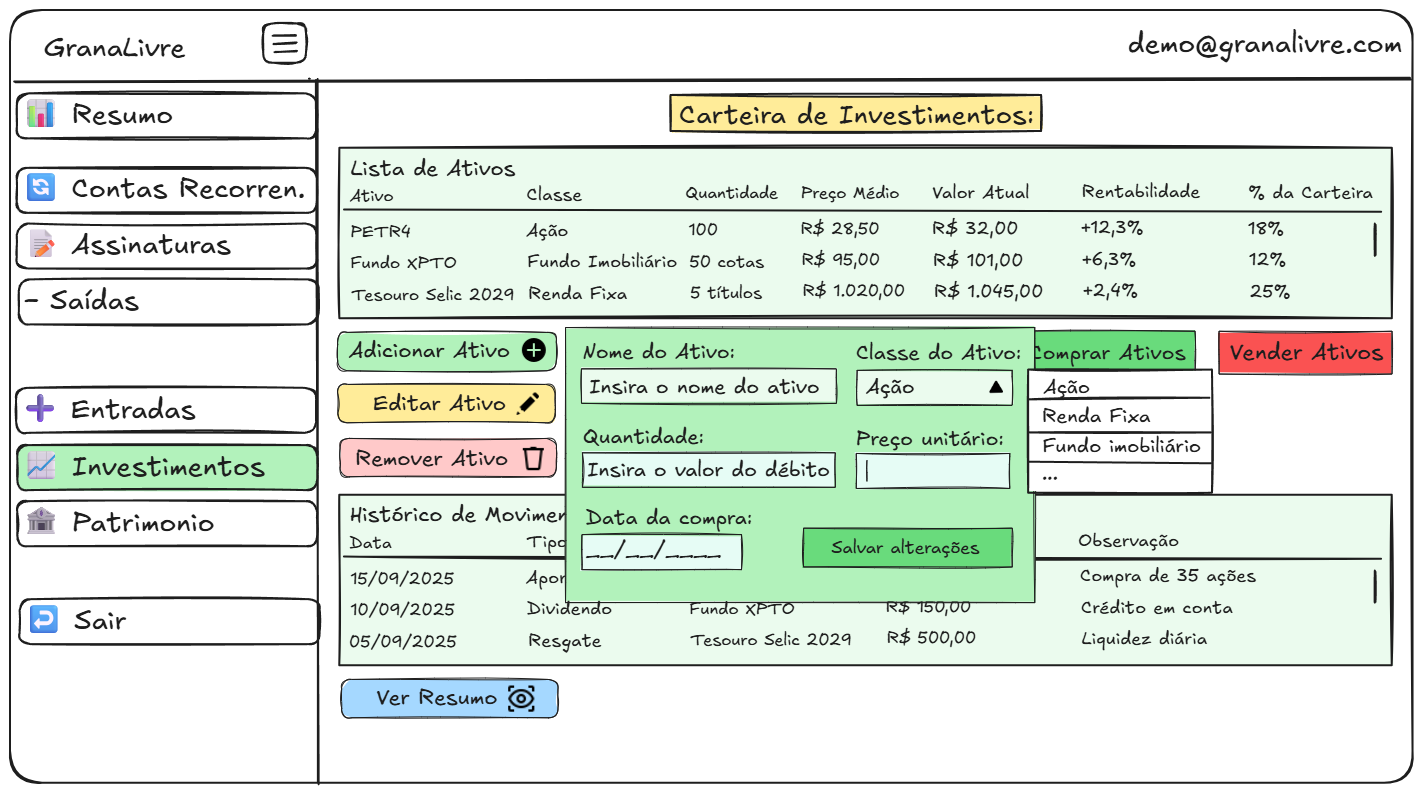
\includegraphics[width=0.9\textwidth]{imgs/08-investimentos_3.png}
    \caption{Protótipo de baixa fidelidade da tela de gerenciamento com o dropdown do botão rescpetivo a adição de um novo ativo}
    \label{fig:prot_investimentos4}
\end{figure}

\begin{figure}[H]
    \centering
    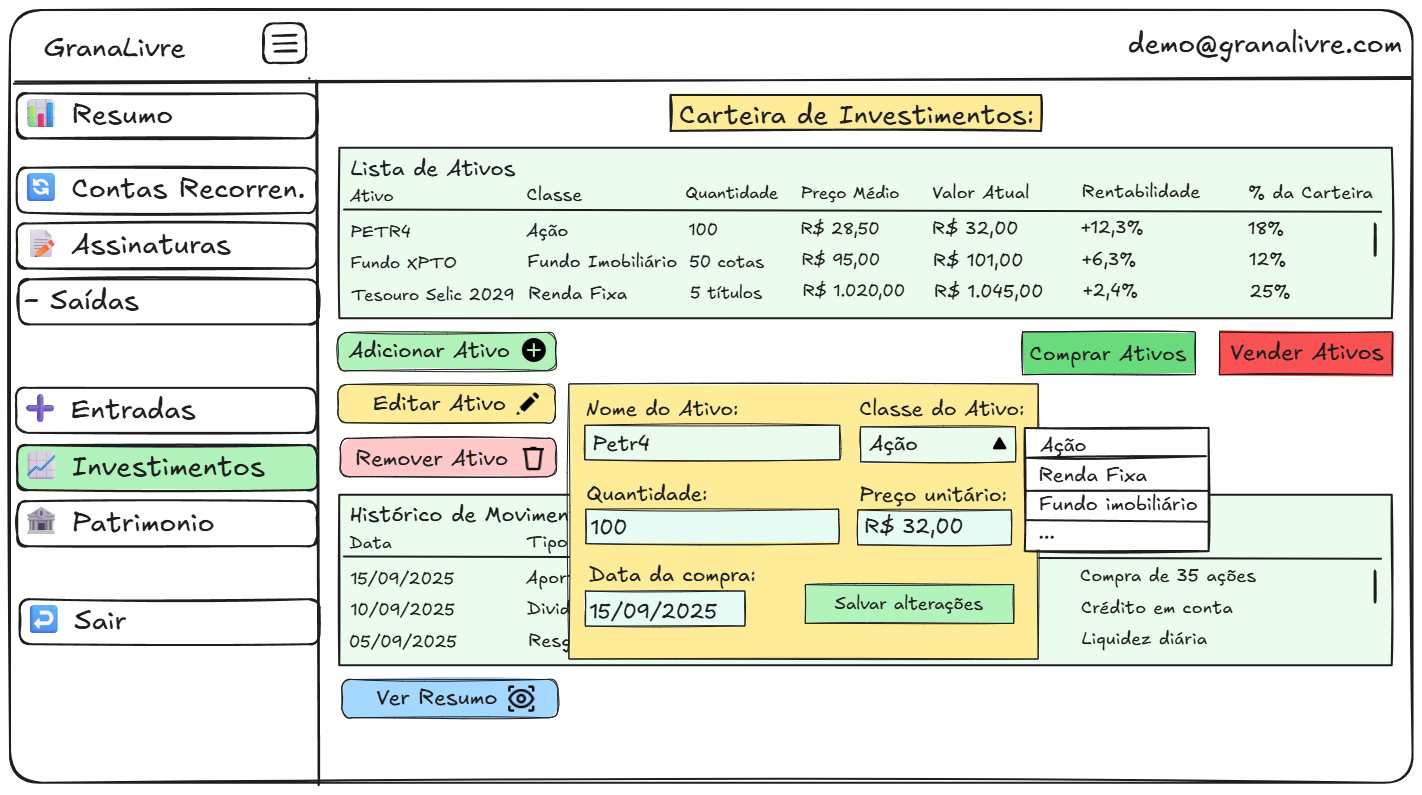
\includegraphics[width=0.9\textwidth]{imgs/08-investimentos_4.png}
    \caption{Protótipo de baixa fidelidade da tela de gerenciamento com o dropdown do botão rescpetivo a edição de um ativo já existente}
    \label{fig:prot_investimentos5}
\end{figure}

\begin{figure}[H]
    \centering
    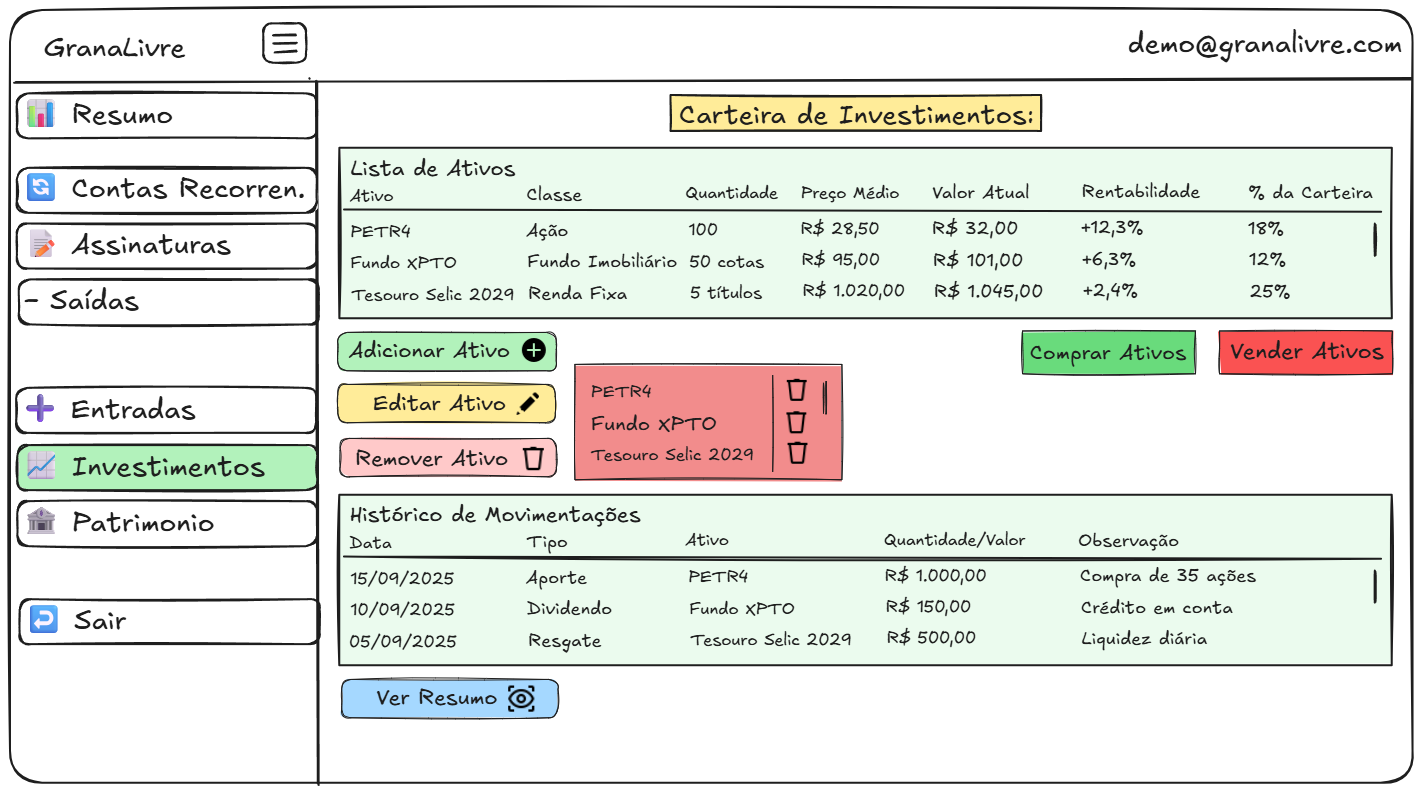
\includegraphics[width=0.9\textwidth]{imgs/08-investimentos_5.png}
    \caption{Protótipo de baixa fidelidade da tela de gerenciamento com o dropdown do botão rescpetivo a remoção de um ativo já existente}
    \label{fig:prot_investimentos6}
\end{figure}

%08-patrimonio.png até 08-patrimonio6.png
\begin{figure}[H]
    \centering
    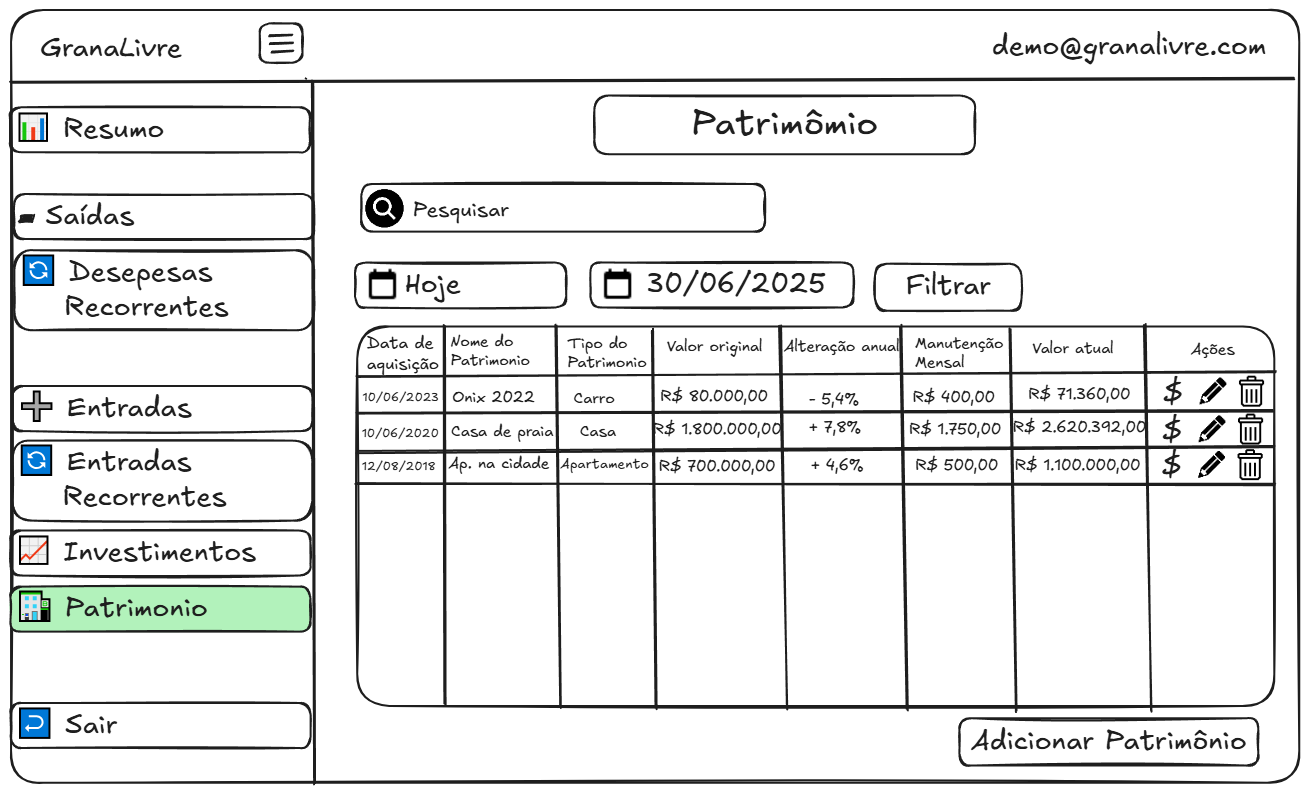
\includegraphics[width=0.9\textwidth]{imgs/09-patrimonio.png}
    \caption{Protótipo de baixa fidelidade da tela de gerenciamento de patrimônio}
    \label{fig:prot_patrimonio}
\end{figure}

\begin{figure}[H]
    \centering
    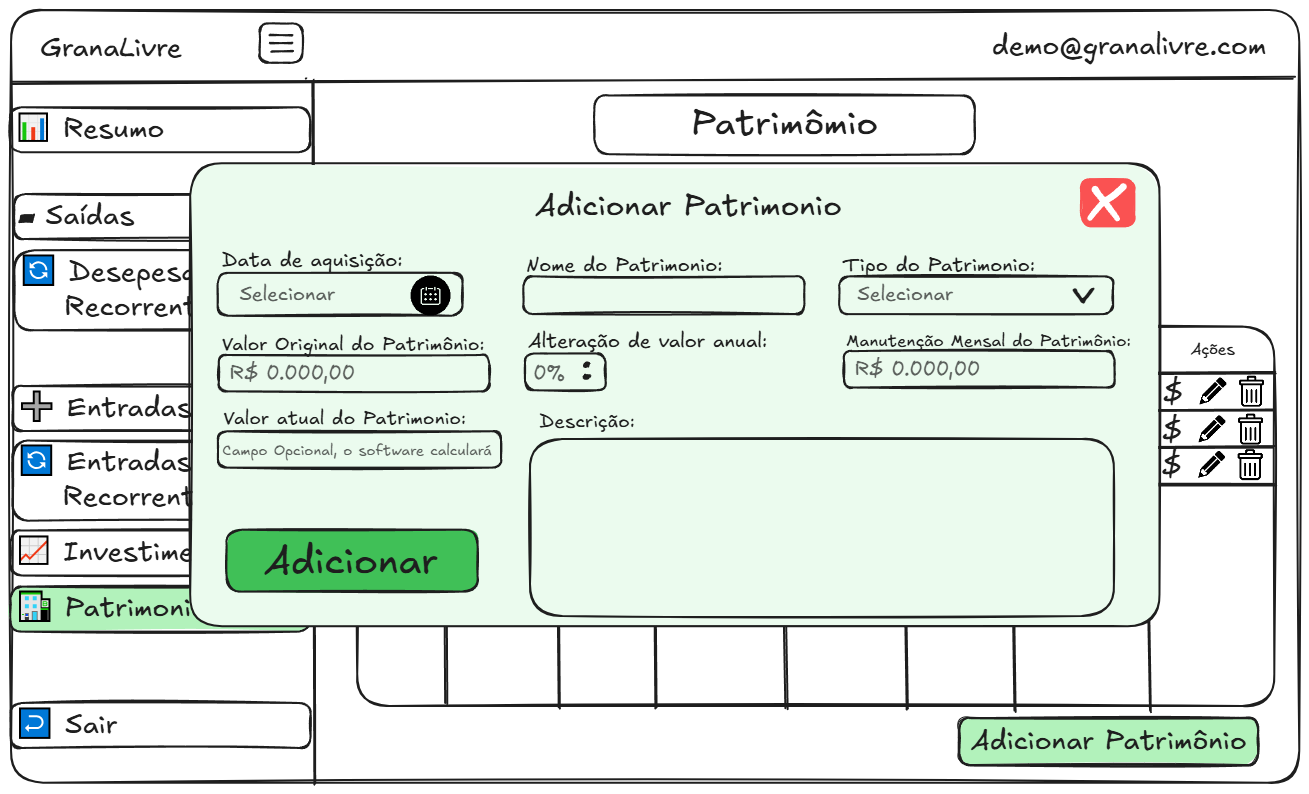
\includegraphics[width=0.9\textwidth]{imgs/09-patrimonio2.png}
    \caption{Protótipo de baixa fidelidade da tela de gerenciamento de patrimônio com formulário para adicionar novo bem}
    \label{fig:prot_patrimonio2}
\end{figure}

\begin{figure}[H]
    \centering
    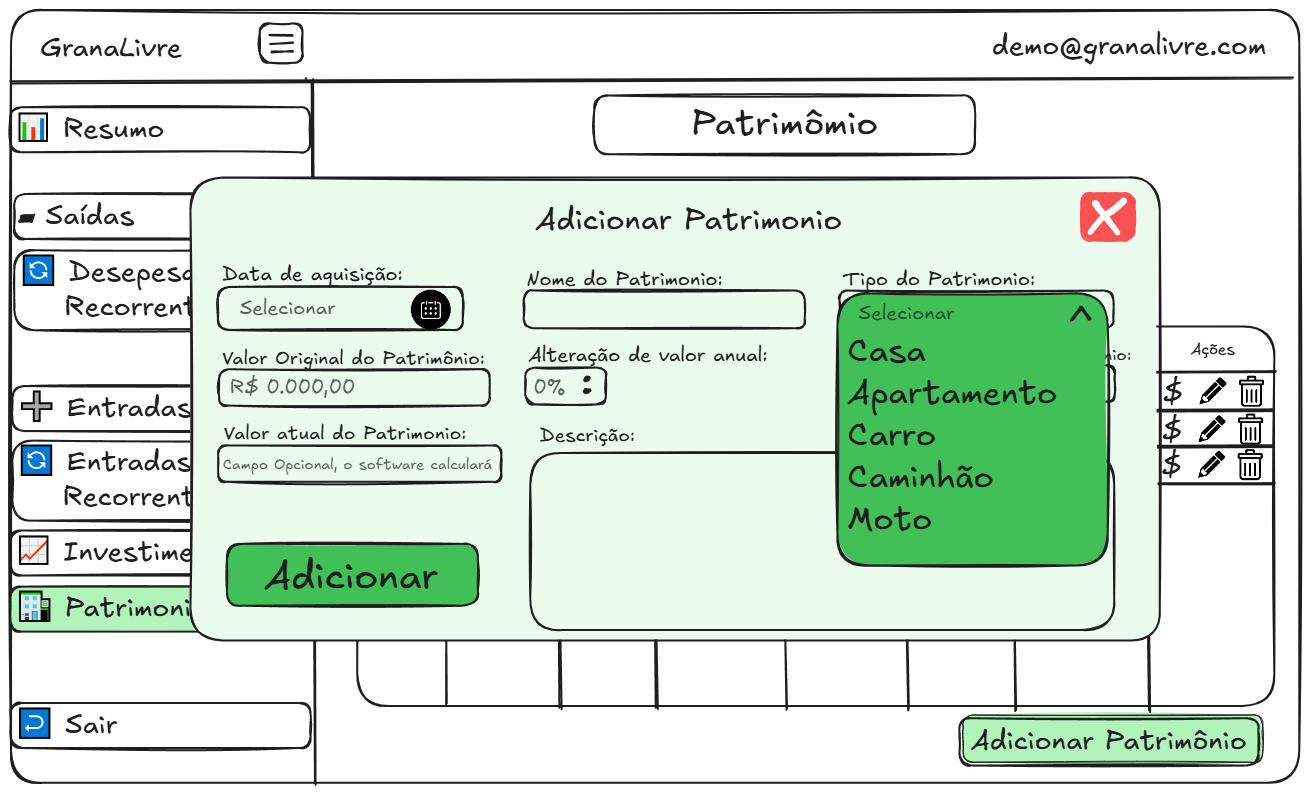
\includegraphics[width=0.9\textwidth]{imgs/09-patrimonio3.png}
    \caption{Protótipo de baixa fidelidade da tela de gerenciamento de patrimônio com menus dropdown ao adicionar novo bem}
    \label{fig:prot_patrimonio3}
\end{figure}

\begin{figure}[H]
    \centering
    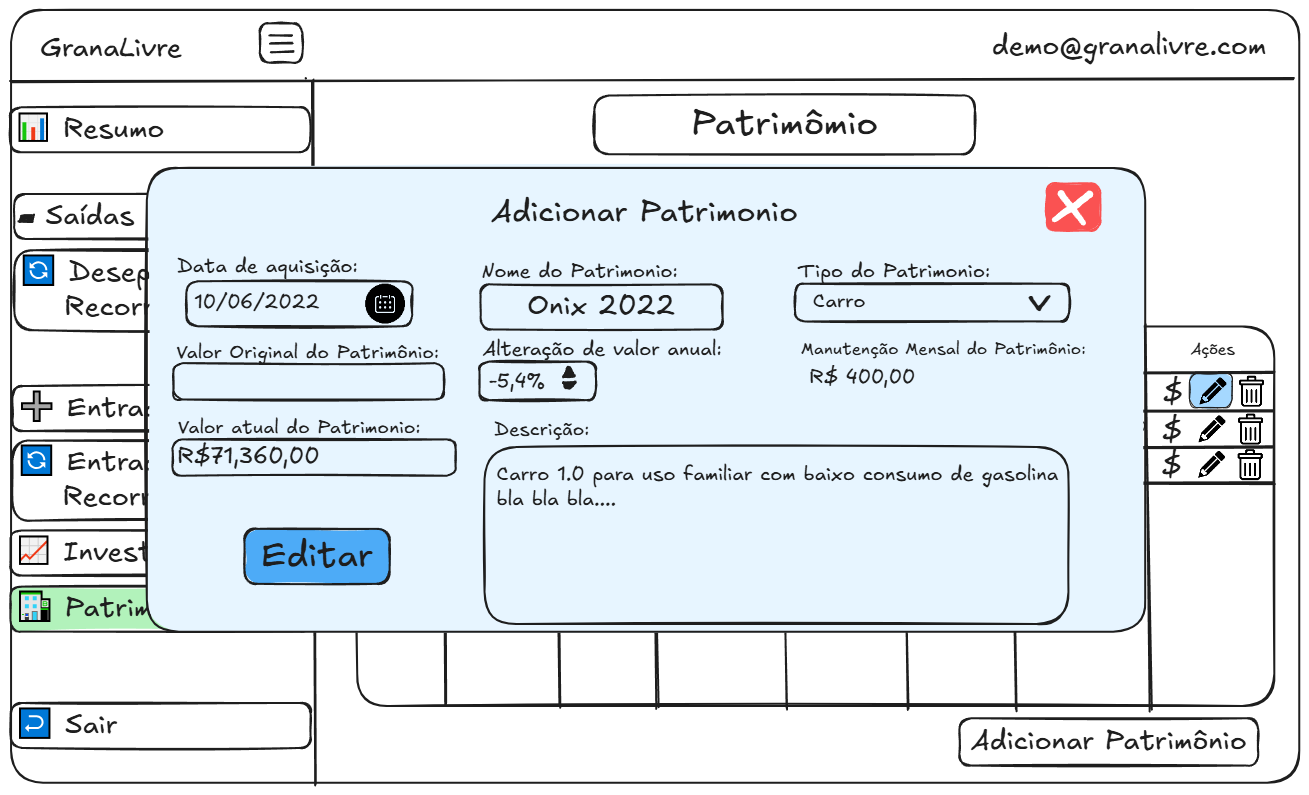
\includegraphics[width=0.9\textwidth]{imgs/09-patrimonio4.png}
    \caption{Protótipo de baixa fidelidade da tela de gerenciamento de patrimônio com formulário para editar um bem existente}
    \label{fig:prot_patrimonio4}
\end{figure}

\begin{figure}[H]
    \centering
    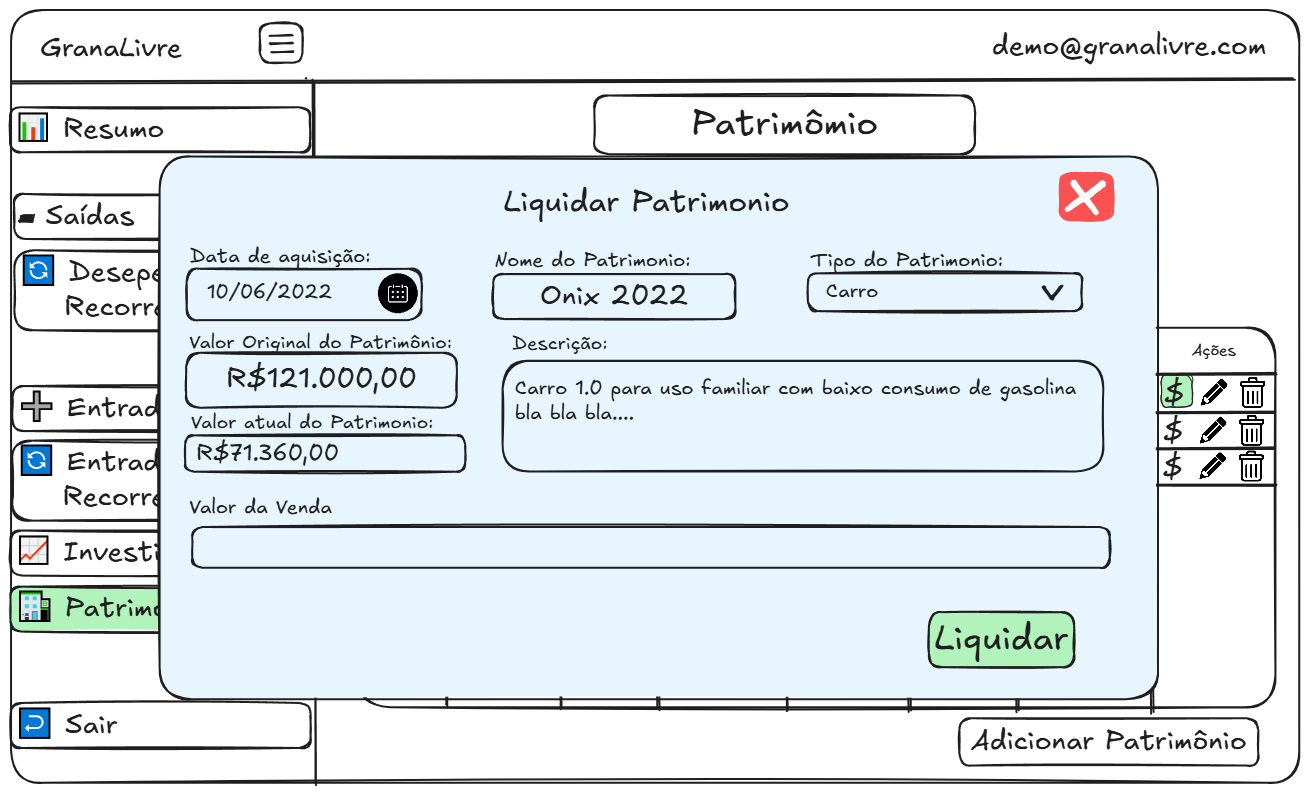
\includegraphics[width=0.9\textwidth]{imgs/09-patrimonio5.png}
    \caption{Protótipo de baixa fidelidade da tela de gerenciamento de patrimônio com formulário para liquidar um bem existente}
    \label{fig:prot_patrimonio5}
\end{figure}

\begin{figure}[H]
    \centering
    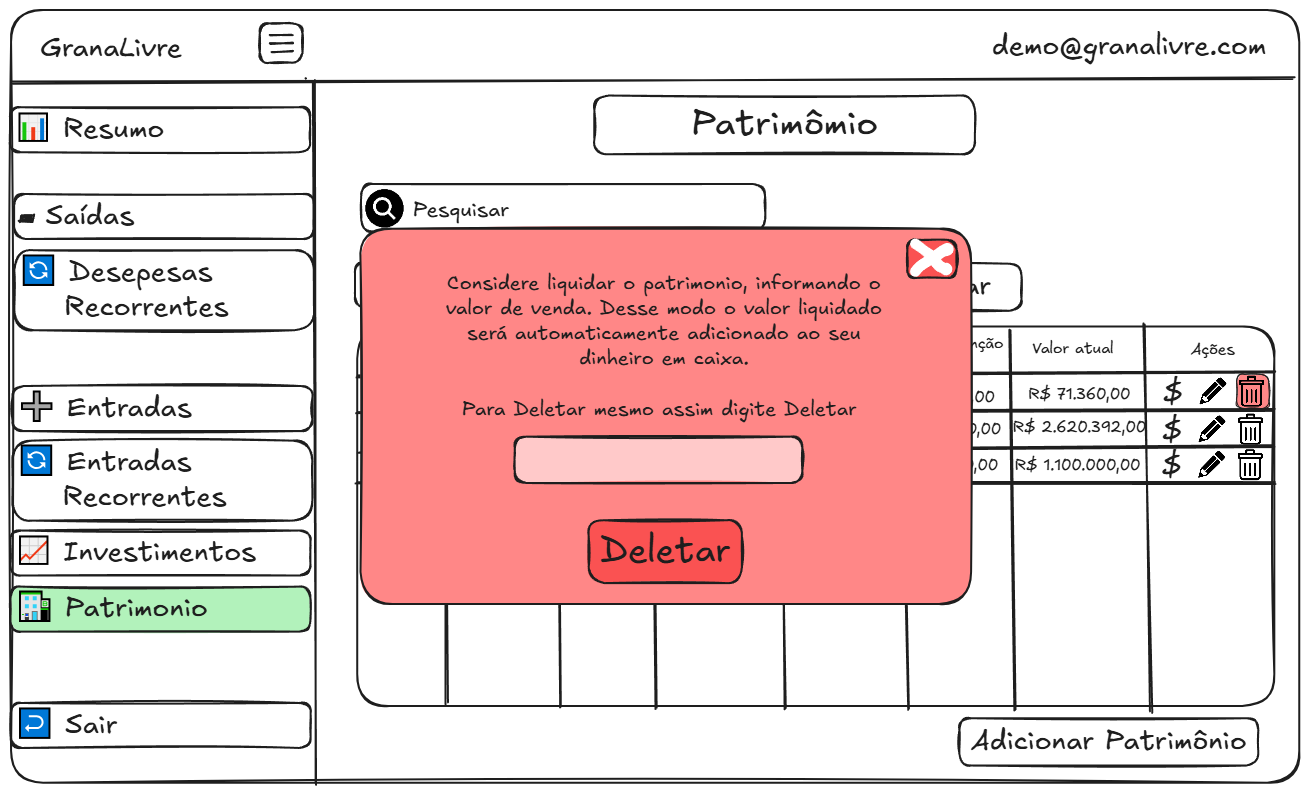
\includegraphics[width=0.9\textwidth]{imgs/09-patrimonio6.png}
    \caption{Protótipo de baixa fidelidade da tela de gerenciamento de patrimônio com confirmação para exclusão de um bem existente}
    \label{fig:prot_patrimonio6}
\end{figure}

% Adicionar outras telas conforme necessário

\section{Diagrama Relacional do Banco de Dados}
A modelagem do banco de dados foi realizada com o objetivo de estruturar as entidades fundamentais para o funcionamento do sistema, assegurando integridade referencial e eficiência nas consultas. O diagrama relacional reflete as tabelas e os relacionamentos definidos.

% \begin{figure}[H]
%     \centering
%     \includegraphics[width=0.9\textwidth]{imagens/der.png}
%     \caption{Diagrama Relacional do Banco de Dados}
%     \label{fig:der}
% \end{figure}